
\section{Royalties}
\crt{861(a)(4); 871(a)(1), (a)(1)(D); 881(a)(1), (a)(4); 1441(a) and (c)(5); and 1442(b)(2)}{1.871-7(b)(1)}{Article 12}

Royalties are U.S. source if they are received for the use of property in the U.S.  \S 861(a)(4).  Thus, the residence of the payor, the owner of property, and the place of payment are irrelevant for sourcing purposes.  U.S. source royalties are FDAP and subject to a flat 30\% tax, but are deductible by the payor if the intellectual property is used in a trade or business.  As we will see below, in situations where income is derived from intellectual property that is produced by personal services, it is not clear whether the income received is royalties or compensation for services.  In addition, it is sometimes difficult to determine whether a transfer constitutes a license producing royalties or a sale producing capital gains.  The U.S. tax consequences can vary greatly depending on the characterization of the income.  Because the United States has historically been a net exporter of intellectual property, it has championed a low or zero rate of source country taxation of royalties.  \textit{See} Article 12.  

Since royalties are deductible by the payor if the property is used in a U.S. trade or business, it is possible to reduce source basis taxation by licensing intellectual property into the source country.  If the royalties are not taxed by the source country when paid, a significant amount of U.S. income could be extracted tax-free by royalties.  Intellectual property is often more difficult to value than other types of property because it is difficult to find property that is comparable:  with what would you compare the Nike swoosh trademark or a patent for a novel drug?  Consequently, related parties (think parent-subsidiary relation) might choose to set the royalty rate at a level that eliminates much source basis taxation.  The same issue arises with inter--company debt, but because there is competition among banks and other suppliers of debt capital, it is much easier to determine if an interest rate is reasonable than if a royalty rate is truly an arm's length rate. We will explore these issues and the responses of governments  when we study section 482 in Chapter 13.   

If a payment is properly characterized as a royalty, its source will be determined based on where the underlying intellectual property was used.  At times, this determination can be challenging.  For example, assume a company licenses a patent to a particular chemical to another company to be used in manufacturing another product.  The patent is used where the particular chemical is produced, where the final product is manufactured, where the final product is sold to distributors, and finally, where the final product is sold to consumers.  Each of these locations has arguably some economic nexus to the revenues produced by the final sale of the product, and an argument could be made to source some of the revenues to each of these locations.  Rev.\@\@ Rul.\@\@ 68-443 addresses this issue.  

Under Article 12, the source country is generally prohibited from taxing royalties.  Such a provision clearly favors countries that develop and export intellectual property, and since the United States has historically been a developer and exporter of intellectual property, most U.S. tax treaties usually have a zero rate on royalties.  The argument for prohibiting source basis taxation is that the expenses incurred in creating the property have been deducted in the residence country and therefore the residence country should have primary jurisdiction over the income generated by these expenses.  Developing countries where the intellectual property is exploited take a different view.  They argue that they should have primary tax jurisdiction over royalty income because the intellectual property is being exploited within their jurisdiction.  Even where countries agree on a method for taxing intellectual property, many challenges arise for tax administrators as it is often difficult to determine if the licensing rate is arm's length as required by section 482 and Article 12, par. 4.

\addcontentsline{toc}{section}{\protect\numberline{}Rev.\@\@ Rul.\@\@ 68-443}
\begin{select}
\revrul{Rev.\@\@ Rul.\@\@ 68-443 }{1968-2 C.B. 304}
\ldots\\
Advice has been requested whether the place of initial sale of a product that bears a trademark is the controlling factor 
in the determination of the source of the royalties paid for the use of the trademark under the circumstances described. 

X, a resident foreign corporation, owns a trademark for certain products in many foreign countries. X corporation 
entered into a license agreement with Y, a domestic corporation, pursuant to which Y was given the right to place the 
foreign trademark owned by X on Y's products and sell the trademarked products. The United States trademark for 
these products is owned by Z, an unrelated party. The license agreement between X and Y is a conventional trademark 
license agreement for a limited period of time and includes customary provisions to identify and protect the licensor's 
proprietorship of this mark. Under the terms of the license, Y corporation pays X corporation a royalty measured 
by a percentage of the initial sales price of the trademarked products. 

Y manufactures the trademarked products in the United States and sells them to foreign buyers in the United States 
for resale and consumption in foreign countries; all rights, title, and interest of Y in the products pass to the foreign 
buyers within the United States. Thus, the initial sale of the trademarked products is regarded as having taken place in 
the United States. 

The specific question presented is whether, by reason of the initial sale of the products to the foreign buyers in the 
United States, Y corporation has ``used'' the foreign trademark in the United States and the royalties paid by Y to X are 
income from sources within the United States.
 
Section 861(a)(4) of the Internal Revenue Code of 1954 states, in part, that royalties for the use of or for the privilege 
of using in the United States trademarks and other like property shall be treated as income from sources within the United 
States. 

Section 862(a)(4) of the Code states, in part, that royalties for the use of or for the privilege of using without the United 
States trademarks and other like properties shall be treated as income from sources without the United States.  The gist of a trademark is its association in the public mind with the product, it being the identifying mark of the trade. 
Ambrosia Chocolate Co. v.\@ Ambrosia Cake Bakery, Inc., 165 F.2d 693, at 697 (1947). 

The function of a trademark is to designate the goods as the product of a particular trader and to protect his goodwill 
against the sale of another's product as his. J.S. Tyree Chemist, Inc. v.\@ Thomo Borine Laboratory, 151 F.2d 621, at 623 
(1945).
 
In the instant case the character of X corporation's income is royalty income measured by a percentage of the sales of 
the foreign trademarked products. The initial sale of the trademarked products to foreign shippers is a means of placing
the products in the avenues of commerce with a view towards their ultimate consumption outside the United States. 
Although the amount of the royalty income is measured by the sales of the trademarked products, the place of sale does 
not necessarily determine the source of such royalty income. 

Since Z owns the United States trademark to these products, the products manufactured by Y and identified 
by the trademark under the license from X cannot be sold in the United States for consumption in the United States. 
Moreover, the foreign countries do not protect the foreign trademarks in the United States. It is concluded, therefore, that 
the royalties paid by Y to X are paid for the use of the trademarks in the foreign countries and that the place of initial 
sale of the trademarked products is not the controlling factor in the determination of the source of income. 

Accordingly, in the instant case, where products are ultimately used in the foreign country where their trademark is 
protected, a royalty, received by X for the use of the foreign trademark, is income from sources outside the United States 
despite the fact that the initial sale of the trademarked articles took place in the United States.
\end{select}

\begin{center}
\textbf{Cascading Royalties}
\end{center}
Consider the case where foreign company A licenses the world-wide rights to a patent to foreign company B, which in turn, sublicenses the U.S. rights to U.S. company C.  When company B pays its royalty comprised of the royalties from many sublicenses to company A, should a part of the royalty be considered U.S. source?  Remember, section 861(a)(4) treats as U.S. source royalties paid for the use of intellectual property in the United States; the identity of the payor is irrelevant.  What if companies A and B are related parties, and company A is not a treaty resident, but company B is?  In Rev.\@\@ Rul.\@\@ 80-362, the IRS held that the royalties from company C to company B and from company B to company A were U.S. source.  Does section 861(a)(4) support this view?  What if no treaty applied to the first royalty payment?    

In \emph{SDI Netherlands B.V. v.\@ CIR}, 107 T.C. 161 (1996), the Tax Court rejected the IRS's position in Rev.\@\@ Rul.\@\@ 80-362.  In reading the case, try to find the exact basis on which the court concluded that United States could not tax the second royalty payment.  Did they specifically conclude that such royalties are not U.S. source under section 861(a)(4)?  If so, on what basis?     

\addcontentsline{toc}{section}{\protect\numberline{}Rev.\@\@ Rul.\@\@ 80-362} 
\begin{select}
\revrul{Rev.\@\@ Rul.\@\@ 80-362 }{1980-2 C.B. 208}
\ldots\\
\begin{center} \textbf{ISSUE}
\end{center} 
Are royalties paid for the use of a patent in the United States, under the circumstances described below, subject to 
United States tax? 
\begin{center} \textbf{FACTS}
\end{center}
A, a citizen and resident of a country other than the United States or the Netherlands, licenses the United States rights 
on a patent to X, a Netherlands corporation. X is a bona fide corporation unrelated to A. X agrees to pay A a fixed royalty 
each year in return for the patent license. X relicenses the patent to Y , a United States corporation, for use in the United 
States. Y agrees to pay X royalties based on the number of units produced by Y each year under the patent. X's fixed 
royalty to A is not contingent upon the receipt of royalties from Y. A's royalty income is not effectively connected 
with the conduct of a trade or business within the United States within the meaning of section 871(b) of the Internal 
Revenue Code. 

Article IX(1) of the United States--Netherlands Income Tax Convention, T.D. 5778, 1950--1 C.B. 92, as amended by 
the United States--Netherlands Supplementary Income Tax Convention, 1967--2 C.B. 472, provides that royalties paid 
to a resident or corporation of the Netherlands shall be exempt from tax by the United States. There is no income tax 
convention between A's country of residence and the United States. 
\begin{center} \textbf{LAW AND ANALYSIS}
\end{center}
Section 861(a)(4) of the Code provides that royalties for the privilege of using a patent in the United States are treated as income from sources within the United States. 

%Section 871(a)(1)(A) of the Code imposes a tax of 30 percent of the amount received from sources within the United 
%States by a nonresident alien individual as interest, dividends, rents, salaries, wages, premiums, annuities, compensations, 
%remunerations, emoluments, and other fixed or determinable annual or periodical gains, profits, and income. 

%Section 1.871-7(b) of the Income Tax Regulations provides that royalties, including royalties for the use of a 
%patent, constitute fixed or determinable annual or periodical income to which the 30--percent tax rate imposed by section 
%871(a)(1)(A) applies. 

%Section 1441(a) of the Code provides that all persons, in whatever capacity acting, having the control, receipt, custody,
%disposal or payment of any of the items of income specified in section 1441(b) (to the extent that any of such items 
%constitute gross income from sources within the United States), of any nonresident individual shall deduct and withhold 
%from such items a tax equal to 30 percent thereof. 

%Section 1.1441-2(a) of the regulations provides that royalties are included in the items of income enumerated under 
%section 1441(b) of the Code. 

In the present factual situations, the royalties from Y to X are exempt from United States tax under Article IX(1) of 
the Convention. However, the royalties from X to A are not exempt from taxation by the United States because there is 
no income tax convention between A's country of residence and the United States providing for such an exemption. Since 
the royalties from X to A are paid in consideration for the privilege of using a patent in the United States, they are 
treated as income from sources within the United States under section 861(a)(4) of the Code and are subject to United 
States income taxation under section 871(a)(1)(A). 
\begin{center} \textbf{HOLDING}
\end{center} 
Royalties paid by X to A are subject to United States tax at the 30--percent rate pursuant to section 871(a)(1)(A) of the 
Code. X , under section 1441(a), is required to withhold from the royalties paid to A a tax equal to 30 percent of such 
royalties.
\end{select}
\addcontentsline{toc}{section}{\protect\numberline{}SDI Netherlands B.V. v.\@ CIR} 
\begin{select}
\caseart{SDI Netherlands B.V. v.\@ CIR}{ 107 T.C. 161 (1996) }{TANNENWALD, Judge}
\ldots
\begin{center} \textbf{Background}
\end{center}
Petitioner is a foreign corporation organized in 1974 under the laws of the Kingdom of The Netherlands. \ldots

During the years in issue, petitioner was a member of an affiliated group of companies (the SDI Group) whose 
members designed, manufactured, marketed, and serviced commercial systems software for use on IBM mainframe computers worldwide. 

SDI Ltd., a corporation organized under the laws of Bermuda, is the parent company of the SDI Group. During the years in issue, petitioner was a wholly owned subsidiary of SDI Antilles, a Netherlands Antilles corporation, which was a wholly owned subsidiary of SDI Ltd.
 
The SDI Group also included SDI Bermuda Ltd. (SDI Bermuda), a corporation organized under the laws of Bermuda which, during the years in issue was a wholly owned subsidiary of SDI Ltd. 

SDI USA, Inc. (SDI USA), a corporation organized under the laws of the State of California was, during the years at issue, a wholly owned subsidiary of petitioner. \ldots  

\ldots

\begin{figure}[hbtp]
\caption{SDI Netherlands v.\@ CIR}
\begin{center}
\setlength\fboxsep{0pt}
\setlength\fboxrule{0.5pt}
\fbox{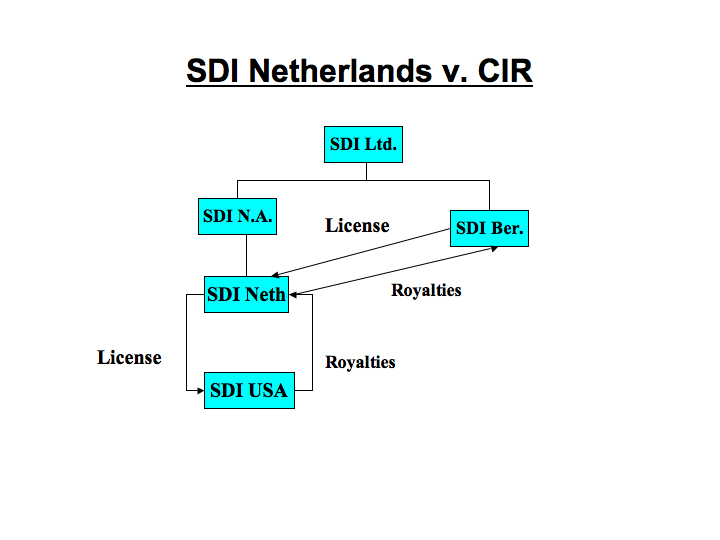
\includegraphics[width=140mm, height=80mm, clip, trim= 5mm 5mm 5mm 20mm]{SDI.png}}
\end{center}
\label{SDI}
\end{figure}

SDI Ltd. provided management services to certain of its direct and indirect subsidiaries for which such subsidiaries paid it management fees. 

\begin{center} \textbf{Royalty Payments Made By Petitioner}
\end{center}
During the years in issue, petitioner licensed from SDI Bermuda, pursuant to a license agreement dated 
November 28, 1986 (Bermuda license agreement), the worldwide rights to certain commercial systems software for use on IBM mainframe computers (the software). The Bermuda license agreement granted petitioner a nonexclusive license to use or to market the use of, on a worldwide basis, all of the software and any and all industrial and intellectual property rights SDI Ltd. had or would acquire from the effective date of the agreement \ldots, in exchange for certain royalty payments. The agreement further provided that petitioner ``shall specifically have the right to grant sublicenses and Agents for the right to use and to market the use of any and all marketing rights granted to [petitioner] under the terms'' of the agreement. The agreement was valid for an indefinite period and could be unilaterally terminated by either party on 3 months' written 
notice. 

The Bermuda license agreement contained no express reference to the United States. 

With respect to royalties, the Bermuda license agreement provided:
\begin{quote} 
8.1 The royalties payable to [SDI Bermuda] by [petitioner] under this Agreement are fixed at 93\% of 
the net amount of all of the royalties due to [petitioner] by all persons, entities and institutions which 
[petitioner] sublicensed any of the rights licensed to [petitioner] under this Agreement (``Sublicensees''). The 
aforementioned net amount is the amount that remains after the deduction of the withholding tax on royalties 
to be withheld when the Sublicensees of [petitioner] or Agents of [petitioner] pay the royalties due to the 
[petitioner].

[The 93\% rate was increased to up to 98\% if the royalties exceeded certain amounts.] 

\ldots
\end{quote} 
[From 1987 through 1990, SDI Netherlands paid between \$3.5 million and \$5.4 million annually to SDI Bermuda.  Those payments constituted roughly 94\% of the total worldwide royalty payments received by SDI Netherlands.]

\begin{center} \textbf{Royalty Payments Received by Petitioner from SDI USA }
\end{center}
During the years in issue, petitioner was a party to an exclusive license agreement with SDI USA, dated October 1, 
1972, and as modified from time to time, regarding the use and licensing of the software in the United States (the U.S. 
license agreement). \ldots SDI USA was responsible for the direct marketing and sales of the software in the United States. 

The U.S. license agreement provided in part:
\begin{quote} 
2.1 In consideration for the payment of the royalties provided hereunder and the performance of the other 
terms and conditions hereof by [SDI USA], [petitioner] hereby grants and transfers to [SDI USA], upon  the terms and subject to the conditions hereinafter set forth, the exclusive right and license during the Term hereof, to have disclosed to it by [petitioner] and to exploit, use and lease and otherwise obtain the benefit of [the software] within the Territory.

2.2 This Exclusive License shall include, (i) the right to sublicense to others the use and lease of [the 
software] within the Territory, subject, however, to the terms and conditions of this License; and (ii) this 
License shall also include the right and, as hereinafter provided, the obligation of [SDI USA], to provide or 
to provide for the exclusive maintenance, servicing and repair of [the software] within the Territory. * * * 
* * * * 

2.4 The Territory of this License shall mean and be restricted to the continental United States, Hawaii and 
Alaska. 
\end{quote}
Petitioner agreed not to license the software for use or to compete directly or indirectly with SDI USA's exploitation \margit{Should there have been an allocation to the non-compete?}
of the software in the United States during the term of its license to SDI USA. \ldots

Until February 1987, the agreement provided that SDI USA would pay to petitioner ``an annual royalty equal to fifty 
percent (50\%) of the annual gross revenues of [SDI USA] from leasing and sublicensing of [the software], 
without any deductions therefrom except rebates, discounts and sales or value added taxes.''
 
The U.S. license agreement was modified in February 1987 to provide that SDI USA would pay petitioner ``a royalty 
equal to (50\%) fift[y] percent of the gross billable or invoiced revenues of [SDI USA] with regard to all products licensed 
herein or further licensed in the future, without any deductions therefrom except rebates, or, sales or value added taxes.'' 

[SDI Netherlands received annual royalty payments from SDI USA from 1987-1990 of roughly \$2.5 million annually.]

\ldots 
 
\begin{center} \textbf{Discussion}
\end{center}
\ldots
\begin{center} \textbf{Liability for Withholding }
\end{center}

Section 881(a) provides that a 30-percent tax shall be imposed on ``the amount received from sources within the 
United States by a foreign corporation'' falling within certain categories of income. \ldots Section 1442 provides a method 
for collecting that tax. 

\ldots 
%Section 1442 provides in part:
%\begin{quote} 
%(a) General Rule.--In the case of foreign corporations subject to taxation under this subtitle, there shall 
%be deducted and withheld at the source in the same manner and on the same items of income as is provided 
%in section 1441 a tax equal to 30 percent thereof. * * *
%\end{quote} 
%Royalties are among the types of income included in section 1441(b). Sec. 1.1441-2(a), Income Tax Regs.; see also 
%sec. 1.881-2(b), Income Tax Regs. In addition, section 861(a)(4) provides that U.S. source income includes:
%\begin{quote} 
%(4) Rentals and Royalties.--Rentals or royalties from property located in the United States or from any 
%interest in such property, including rentals or royalties for the use of or for the privilege of using in the United
%States patents, copyrights, secret processes and formulas, good will, trade--marks, trade brands, franchises, 
%and other like property.
%\end{quote} 
%Section 1441(a) completes the picture of the statutory provisions involved herein. It provides: 
%\begin{quote}
%all persons * * * having the control, receipt, custody, disposal, or payment of any of the items of income 
%specified in subsection (b) [which includes ``royalties''] (to the extent that any of such items constitutes 
%gross income from sources within the United States), of any nonresident alien individual or of any foreign 
%partnership shall * * * deduct and withhold from such items a tax equal to 30 percent thereof * * * 
%\end{quote}
There can be no dispute that the royalty payments received by petitioner from SDI USA constitute U.S. source income and were received by petitioner as such within the meaning of section 1442(a). \ldots There is no comparable U.S. treaty exemption that would apply to royalty payments from SDI USA to SDI Bermuda. 

The parties have locked horns on several aspects of the application of the statutory provisions in light of the impact of 
the U.S.--Netherlands treaty exemption: (1) Whether the royalties paid by petitioner to SDI Bermuda constitute income 
``received from sources within the United States by'' SDI Bermuda and are thus subject to withholding under section 
1441(a);\ldots

%(2) whether petitioner can be considered a ``withholding agent''; (3) whether there is a limitations period that 
%has expired in respect of respondent's right to assess a deficiency in withholding tax against petitioner; and (4) whether 
%petitioner is liable for additions to tax under section 6651(a)(1) for failure to file withholding tax returns. 

For reasons hereinafter set forth, we resolve the first issue in petitioner's favor with the result that it is unnecessary for 
us to address the remaining issues. \ldots Before proceeding with our analysis of the first issue, however, it is important to 
note that respondent does not question the existence of petitioner as a valid Netherlands corporation or the application of 
the treaty exemption insofar as the payments by SDI USA to petitioner are concerned. Similarly, respondent does 
not attack the arrangements under which petitioner had a license of the worldwide rights and SDI USA had a license of 
the U.S. rights, although respondent does ask us to take into account the close relationship of the various corporations 
involved. \ldots

Rather, respondent focuses her argument solely on the proposition that, since the royalties paid by SDI USA to 
petitioner were U.S. source income, they retained that character as part of the royalties paid by petitioner to SDI 
Bermuda and, as a matter of law, constitute income ``received from sources within the United States by'' SDI Bermuda 
under section 881(a). \ldots Respondent contends that the fact that such royalties were combined with non--U.S. source 
royalties  received by petitioner to determine the amount of royalties payable by petitioner to SDI Bermuda 
does not preclude the tracing of the royalties received by petitioner from SDI USA to U.S. sources. \margit{The IRS argues that royalties do not change source when paid through chains of sublicensees.} To implement such 
tracing, respondent simply applies the percentage specified in the worldwide license agreement between petitioner and 
SDI Bermuda and utilized in computing the amount of the required payment by petitioner to SDI Bermuda. \ldots In all of [the cases cited by the CIR], however, the payments, upon which a 
withholding tax was imposed, were directly from a U.S. payor and the U.S. withholding tax was imposed on that payor. 
None of them address the situation involved herein, where there is a second licensing step under which royalties are being 
paid and upon which the U.S. withholding tax is sought to be imposed. Thus, these cases provide no guidance in respect
of whether the U.S. source characterization of the royalties paid by SDI USA to petitioner flows through to the royalties 
paid by petitioner to SDI Bermuda. 

Petitioner argues that the royalties paid by SDI USA to petitioner and exempt from tax under the Netherlands treaty 
became merged with the other royalties received by petitioner from non--U.S. sources and consequently lost their character 
as U.S. source income. Petitioner submits that, while the royalty payments from SDI USA may be U.S. source 
income, its royalty payments to SDI Bermuda were made on a separate and independent basis. With respect to the 
payments to SDI Bermuda, petitioner contends that they were made pursuant to a worldwide licensing agreement between 
two foreign corporations, and as such do not constitute income ``received from sources within the United States'' so that 
no withholding is required under section 1442(a). 
Pertinent authority on the issue before us is sparse. Indeed respondent relies solely on Rev.\@\@ Rev.\@\@ 80--362, 1980--2 C.B. 
208, for her ``flow--through'' position. \ldots 
 
We are not persuaded that Rev.\@\@ Rul.\@\@ 80--362, supra, \margit{Note the lack of deference the Tax Court accords revenue rulings.} provides any significant support for respondent's position herein. It 
fails to reflect any reasoning or supporting legal authority. This circumstance is particularly relevant in applying the usual 
rule that, in any event, revenue rulings are not entitled to any special deference. \ldots 
 
At this point, we note that respondent has not argued that petitioner was a mere conduit or agent of SDI USA in paying 
royalties to SDI Bermuda or that SDI Bermuda was the beneficial owner of the royalties petitioner received from SDI USA 
so that the U.S.--Netherlands treaty exemption should not apply. \ldots Presumably such an argument would have produced a situation 
where SDI USA rather than petitioner would have been targeted by respondent as the taxpayer liable for the withholding 
tax under section 1442(a). \ldots 

Although [Aiken and Northern Indiana] involved the conduit concept, we think they provide some guidance for our disposition of the instant 
case. We take this view because the flow--through characterization concept is, in a very real sense, the conduit concept 
albeit in a somewhat different garb, i.e., whether the U.S. source income is being received as such, because of the status 
of the paying entity in one case, and the status of the subject matter of the payment in the other.

In [Aiken], back--to--back loans, in the identical amounts of principal and rates 
of interest, were made between a U.S. corporation and a related corporation organized under the laws of the Republic 
of Honduras, and between the Honduran corporation and its indirect parent. Respondent argued that the Honduran 
corporation should be disregarded for tax purposes, and that the parent corporation should be deemed the true owner 
and recipient of the interest payment from the U.S. corporation. We held the Honduran corporation to be a mere 
conduit for the passage of interest payments and imposed withholding tax liability on the U.S. corporation.
 
In [Northern Indiana], the taxpayer, a domestic corporation, organized a 
finance subsidiary incorporated in Curacao under the Commercial Code of the Netherlands Antilles, (to which the U.S.-- 
Netherlands treaty applied) for the purpose of issuing notes in the Eurobond market. The finance subsidiary borrowed 
\$70 million at 17--1/4 percent interest in that market and lent that amount to the taxpayer at 18--1/4 percent interest. 
Respondent argued that the finance subsidiary should be ignored and that the taxpayer was liable for withholding taxes 
under section 1441 on the interest payments to the foreign Eurobond holders. Finding that the finance subsidiary engaged 
in substantive business activity that resulted in significant earnings, we held that the finance subsidiary was not a mere 
conduit or agent. 

We think the within situation falls more within the ambit of Northern Indiana than Aiken Industries. In the 
latter case, there was an identity both in terms and timing between the  back to back loans, as well as a close 
relationship between the parties involved. In the former case, although there was a clear connecting purpose between 
the borrowing and lending transactions, \emph{i.e.}, to obtain the benefit of the exemption from the withholding tax on interest 
under the U.S.--Netherlands treaty; there were differences in terms, \emph{i.e.}, in the interest rate (albeit not large); and a close 
relationship between all the parties was not present since the borrowings by the finance subsidiary were from unrelated 
parties. 

In the instant case, there was a close relationship between the parties. However, although respondent asks us, in 
passing, to take that relationship into account, she does not pursue the matter to the point where she contends that it is a 
significant factor. Given the fact that respondent recognizes the existence of all of the parties as valid corporate entities and 
does not attack the bona fides of the license agreements between SDI USA and petitioner, on the one hand, or petitioner 
and SDI Bermuda, on the other, we are not disposed to allow the close relationship element to control our decision. 

The facts of the matter are that the two license agreements had separate and distinct terms and that petitioner 
had an independent role as the licensee from SDI Bermuda and the licensor of the other entities, including but not 
limited to SDI USA. The schedules of royalty payments provides for a spread, not unlike the spread involved in Northern 
Indiana, which compensated petitioner for its efforts. Like the finance subsidiary in Northern Indiana, petitioner engaged 
in licensing activities from which it realized substantial earnings. In fact, on a percentage basis, it earned between 5 and 6 
percent, compared to the 1 percent earned by that finance subsidiary in Northern Indiana. \ldots Under the circumstances 
herein, we think these arrangements should be accorded separate status with the result that, although the royalties paid 
by petitioner to SDI Bermuda were derived from the royalties received by petitioner from SDI USA, they were \margit{Did the court get sidetracked with the conduit argument?}  
separate payments. 

We find support for our conclusion herein in that respondent's view of the law could cause a cascading royalty 
problem, whereby multiple withholding taxes could be paid on the same royalty payment as it is transferred up a chain of 
licensors. \ldots  But for the U.S.--Netherlands treaty, the royalty 
payments from SDI USA could be subject to withholding tax twice under respondent's reasoning herein. 

Respondent argues that only one withholding tax is being sought herein. However, this ignores the fact that, by 
treaty, the U.S. agreed to forgo taxing royalties and to allow them to be taxed by The Netherlands. Whether or not The 
Netherlands actually taxed the royalties is irrelevant. 
Respondent also infers that she would use her discretion not to apply more than one level of withholding tax on
multiple transfers of income that originated as U.S. source income. We think this  places an improper exercise of 
discretion in respondent's hands. To avoid the imposition of interest and additions to tax as determined by respondent 
herein, each payor in the chain might well feel compelled to file returns and pay withholding taxes. \ldots  We are not disposed to 
conclude, in the absence of any legislative expression on the subject, that Congress intended the statutory provisions to 
permit ``cascading'' with the question of relief left to the mercy of respondent. 

We hold that the payments by petitioner with respect to which respondent seeks to impose liability for the 30 percent 
withholding tax herein were not ``received from sources within the United States by'' SDI Bermuda under sections 881(a), 1441(a), and 1442(a).\footnote[17]{ 
We note that changes in the U.S.--Netherlands treaty, applicable to years subsequent to the years before us, 
may provide a different framework for disposing of this issue. \ldots }

Decision will be entered for petitioner.
\end{select}

In commercial contracts, it is not uncommon to designate an amount as a royalty if it is determined by reference to future sales.  For example, an author can be paid a fixed amount and a ``royalty'' based on the total sales of his book.  This is often an efficient arrangement if the parties cannot agree \emph{ex ante} on the value of the author's service.  The tax issue that arises is whether such an amount is truly a royalty or instead a payment for services.  The following cases, \emph{Ingram v.\@ Bowers} and \emph{Pierre Boulez v.\@ CIR}, address this issue.  What can potentially happen to a taxpayer if one country taxes income as services and the other as royalties?  


\addcontentsline{toc}{section}{\protect\numberline{}Ingram v.\@ Bowers} 
\begin{select}
\caseart{Ingram v.\@ Bowers}{ 47 F.2d 925 (S. D. N. Y. , 1931) }{PATTERSON, Judge}\\

\ldots 

The case concerns the taxability of income received by 
Caruso by reason of the sale of phonograph records outside the United States, it being conceded that the singing 
by Caruso for the manufacture of such records occurred 
within the United States. The plaintiff contends: First, 
that Caruso was a nonresident alien, a proposition which 
the defendant disputes; and, second, that the amounts in 
question were not income from sources within the United 
States, which the defendant also disputes. 

Caruso was the foremost singer of the world. His fame 
was international, although the greater part of his singing 
during the last ten years of his life was done in the United 
States. He was born in Italy and always remained a subject of that country. For many years prior to his death in 
1921, he spent about six months of the year in the United 
States, singing at the Metropolitan Opera House in 
New York City and giving concerts at other cities. At the 
close of the operatic season, he almost always returned 
to Italy, where he maintained a large estate. His headquarters in the United States were the Knickerbocker Hotel, 
New York City, where he leased a suite of rooms, and 
later the Vanderbilt Hotel here. He married the plaintiff 
here in 1918, and in 1919 a daughter was born here. His 
income from opera and concert work in the United States 
was large and in making income tax returns he always 
claimed the status of a nonresident alien. During his lifetime, no question seems to have been raised as to this 
being his real status. 

Among his other engagements, Caruso was under contract with the Victor Talking Machine Company, a New 
Jersey corporation, to sing for the purpose of enabling the 
Victor Company to make phonograph records of selections rendered by him. By contract dated April 3, 1909, 
he agreed to sing selections at the Victor laboratories in 
Camden, the Victor Company to pay him a royalty of 50 
cents on each larger record and a royalty of 25 cents on 
each smaller record of his voice which it should sell. The 
contract was to continue for twenty--five years and 
was exclusive in the sense that Caruso bound himself not 
to sing for the purpose of making phonograph 
records for any one else.\margit{Note the noncompete and failure to allocate any of the payments to the noncompete.} On January 1, 1919, this contract was superseded by a new one, under which Caruso 
was to render forty selections at the Victor laboratories. 
The Victor Company bound itself to pay Caruso a royalty 
equal to 10 per cent. of its list price on all records of his 
voice which should be sold, and it ``guaranteed'' a minimum payment of \$100,000 a year during his life but not 
to exceed ten years. (It may be noted here that for the 
remainder of Caruso's life the royalties on the percentage 
basis were far in excess of \$100,000,\margit{This amount is equivalent to \$1.37 million in 2012 dollars.} so that the ``guaranty'' did not become operative.) The 1919 contract also 
contained a provision to the effect that Caruso would not 
permit any records of his voice to be made by any other 
concern. 

In performance of these successive contracts, Caruso 
would go to Camden and sing operatic selections. The 
sound would be recorded on wax, from which a master matrix would be made. From this master matrix the 
records for sale in the United States were manufactured. 
Records of Caruso's voice were also sold in other 
countries under the Victor contracts, and it is in relation to 
the royalties measured by sales in these countries that the 
present case arises. By contracts with companies doing 
business in Canada and in England, the Victor Company 
agreed to furnish such companies with matrices of its selections. One of the terms as to payment by the foreign 
companies was that they should pay the Victor Company 
all royalties which the latter was called upon to pay the 
artist. Pursuant to such contracts, the Victor Company 
sent various matrices of songs by Caruso to the foreign 
companies, and in due course they credited the Victor 
Company with sums of money representing the royalty 
which the Victor Company was obligated to pay Caruso, 
the amounts depending of course upon the number of 
records sold by the foreign companies. These sums were 
credited to Caruso on the Victor books and were paid to 
him along with the payments for records sold within the 
United States. 

%Upon an audit of Caruso's income tax return for 1918, 
%the commissioner added the sum of \$18,536.25 to his 
%taxable income as the amount received by him from the 
%Victor Company because of the sales of records abroad. 
%The tax thereon was \$13,924.69. Similarly for the 
%year 1919, the sum of \$1,789.75 was added to income, 
%and a further tax of \$1,086.86 was assessed. Similarly for 
%1920, the sum of \$36,400.59 was added to income, and 
%a further tax of \$25,844.42 was assessed. The plaintiff 
%paid these amounts, totaling \$40,855.97, under protest 
%and brought this action to recover them. 
%Section 213(c) of the Revenue Act of 1918 (40 Stat. 
%1066) deals with nonresident aliens and provides that in 
%their case ``gross income includes only the gross income 
%from sources within the United States.''
 
%The first issue is whether Caruso was a resident alien 
%or a nonresident alien during the three years in question. 
%If he was a resident alien, he was taxable upon his entire 
%net income, irrespective of source. But I have no doubt 
%that his status was that of a nonresident. His original residence was in Italy, and there is no satisfactory evidence 
%of an intention to abandon that residence. His stays in the 
%United States were transitory and, except for one or two 
%occasions, were only for the purpose of fulfilling operatic 
%and concert engagements. Granting that domicile and residence are not synonymous under the income tax 
%statutes [Bowring v.\@ Bowers (C.C.A.) 24 F.(2d) 918], I am 
%persuaded that Caruso's residence as well as his domicile 
%was in Italy. He was therefore taxable only on income 
%from sources within the United States. 

The [source of income from the foreign sales] is not so easy of solution. Did the 
moneys received by Caruso on account of foreign sales of 
records constitute income from sources within the United 
States? I have reached the conclusion that they did. The 
contracts which Caruso made with the Victor Company 
were contracts requiring him to render services. They 
called upon him to sing for Victor and to refrain from 
singing for any other phonograph company. For this he 
was to be paid by Victor according to the number of 
records sold, with a minimum compensation to be paid 
in any event. The contracts were in no sense contracts of 
sale or of license. Caruso had no proprietory right, title, 
or interest in the matrices or in the records. It is true that 
compensation was measured, in part at least, by the number of records sold and was referred to as a royalty; but 
the fact remains that the arrangement was one to render 
services in his capacity as a singer, as thoroughly as if the 
compensation had been a set sum.
 
The services rendered by Caruso were rendered in the 
United States. I think that this is the decisive feature. 
Those services were the source of all his income derived 
from the Victor contracts. It cannot be denied that but 
for the sales abroad part of this income would not have 
accrued. An event in a foreign country was necessary 
before the income became payable. But this 
cannot obscure the fact that the source, the origin of the 
income was Caruso's singing in Camden, N.J. I cannot 
see any difference in principle between this case and a 
case where a lawyer performs services in New York on a 
lawsuit pending in London, his compensation to be contingent upon success in the lawsuit. No income is realized 
until the happy issue of the suit in London, but clearly the 
source of the income, when realized, was the work done 
in New York. Or suppose a nonresident alien spends a 
year in New York working as sales manager for a merchandising company, his compensation to be a percentage 
of the proceeds of sales, and part of the sales are made in 
Canada and Mexico. Beyond doubt his earnings represent 
income from sources within the United States, where all 
his work was done, despite the fact that the amount 
of his earnings was enhanced by sales which took place 
in foreign countries. The same is true here. It seems to 
me that where a singer makes and performs in the United 
States a contract to sing for a phonograph company, for 
which he is to be paid a fixed sum for each record sold 
or a percentage of the list price of the records sold, the 
compensation so received is income from sources within 
the United States; the fact that some of the sales were 
made in foreign countries is immaterial. 

\ldots 
%I have considered the cases holding that where a life 
%insurance agent has obtained policies in earlier years, under an agreement with the insurance company that he is 
%to receive a commission out of all renewal premiums on 
%such policies, such commissions received by the agent 
%in later years will be deemed income for the years when 
%received. Edwards v.\@ Keith (C.C.A.) 231 F. 110; Woods 
%v.\@ Lewellyn (C.C.A.) 252 F. 106. These cases stand for 
%the proposition that where a person performs services for 
%compensation conditionally promised, no income is realized until such time as the condition is performed; the 
%time when the work was done is unimportant. The proposition is clearly a sound one and would apply to the present situation if there were any question as to the time 
%when Caruso received income under the Victor contracts. 
%See, also Zimbalist v.\@ Anderson (D.C.) 23 F.(2d) 328, affirmed in (C.C.A.) 38 F.(2d) 57. But here the question is 
%one of place, not of time; the search, under the terms of 
%section 213(c) of the Revenue Act 1918, is for the territorial source of the income. And, as already pointed out, 
%it seems to me that the place where the work is done, and 
%not the place where the later event fixing compensation 
%occurs, is the source of the income, in cases where the 
%income is from the exercise of a profession or vocation as 
%in this case. 

%I have already said that the controlling fact is that 
%Caruso's part in the making of the records was performed 
%in this country. There are, however, other elements in the 
%case which reinforce the conclusion that the source of this 
%income was within the United States. It was the reputation which Caruso had won by his operatic and concert 
%successes in the United States that led to the making of 
%the Victor contracts. It was here that the contracts were 
%made. It was here that the payments under the contracts 
%were made. The payments were the obligation 
%of a company incorporated and doing business here. The 
%fact that the foreign sales were made by other companies 
%is of no consequence; the situation is the same as if Victor 
%had made such sales directly. It would have been accountable to Caruso for the agreed amount or percentage in any 
%event, even if it had received nothing from its contractors 
%in England and Canada. 

My conclusion is that the income was from sources 
within the United States and was therefore taxable. A 
verdict for the defendant is accordingly directed.
\end{select}

\addcontentsline{toc}{section}{\protect\numberline{}Ingram v.\@ Bowers} 
\begin{select}
\caseart{Ingram v.\@ Bowers}{ 57 F.2d 65 (2nd Cir. 1932) }{L. Hand, Circuit Judge}\\

\ldots 

%The case turns upon the meaning of the phrase, ``gross 
%income from sources within the United States,'' as used 
%in section 213(c) of the Revenue Act of 1918 (40 Stat. 
%1066); for we assume arguendo that, as the judge found, 
%Caruso was a non--resident alien. If his agreements with 
%the Victor Company were no more than contracts for personal services, it makes no difference whether we hold, 
%as was held below, that the source of the resulting income 
%was the services rendered,  or the promise to pay 
%the royalties. The first has the authority of a departmental 
%ruling (Cum. Bul. Dec. 1920, p. 128), and whatever infer- 
%ences may be drawn from the amendments in the statutes 
%from 1921 forward (section 217(a)(3) of the Acts of 1921 
%(42 Stat. 244) and 1924 and 1926 (26 USCA � 958(a)(4); 
%� 119(a)(3) of 1928, 26 USCA � 2119(a)(3). On the other 
%hand we find it difficult to distinguish Edwards v.\@ Keith, 
%231 F. 110 (C.C.A. 2) and Woods v.\@ Lewellyn, 252 F. 
%106 (C.C.A. 3). A priori, the source of an income would 
%seem to be determined by the same factors, whether time 
%or place be in question; if that source is the consideration 
%for the promise, and not the promise itself, the return for 
%services rendered before any tax was imposed would not 
%be a gain from any taxable source. However, we are not 
%driven to a decision on this point, because if the source 
%is the promise, the promisor was also within the United 
%States, and the same result follows as though the service 
%was the source. 

The more vital question is whether the contracts were 
for more than personal services; whether they gave to 
Caruso some interest in the matrices and records, or, if 
there was any copyright, in the copyright; and 
whether the payments can in this wise be looked at as 
emanating from property. If so, the plaintiff argues, the 
sums in suit came from the foreign matrices; if not, then 
at least from the foreign companies. As to both matrices 
and records the second contract is too clear for question; 
it provides that Caruso ``grants all rights in and to'' them. 
The first contract contained no such words, but we think 
that the result was the same. In it he only agreed ``to 
make these records,'' meaning of course, to sing into the 
recording apparatus, and the Victor Company, to pay him 
a royalty as records made from the resulting matrices were 
sold. The company was to manufacture both; prima facie 
they became its chattels like anything else of its mak[ing]. If 
it was intended to give Caruso an interest in them, some 
such reservation was to be expected, and there was none. 
The fact that his return was called a royalty is immaterial; 
it was so described in the second contract which was not 
equivocal. No remedy was created by which he could 
assert any such rights. It appears to us that the purpose 
was the same as was expressed later, and if so, he had 
no proprietary interest in the profits arising out of
the records. If there be a copyright under section 1(e) of 
the Copyright Act (17 USCA \S 1(e)---which we 
do not say---it became embodied in the matrices, as a 
literary composition is embodied in its text. Any putative 
monopoly would do no more than prevent the copying 
of these, and it passed with the property in them. It was 
not impliedly reserved separate from them, for that would 
have interfered with their full enjoyment which the manufacturer was certainly to have. 

Nor can we see how the source of the payments could 
be the royalties paid by the foreign companies to the 
Victor Company. They did not promise to pay Caruso, 
or to assume the obligations of the company.Whether in 
the event of its insolvency, he could have had recourse to 
their promises is beside the mark. Assuming as much, 
it would be only as security for the Victor Company's 
performance, and that would not change the source of 
the income while it continued to perform. For argument 
we may even assume the contrary after default; it never 
did default; all the payments here in question came from 
it. This would be equally true, though by a long stretch 
we were to assimilate the situation to that in Re Waterson, Berlin \& Snyder Co., 48 F.(2d) 704 (C.C.A. 2), and hold that Caruso had a lien upon the matrices sent 
to the foreign companies. That would again be only as 
security, for under the doctrine of that decision the second assignee does not, by accepting the transfer, become 
personally liable on the promise of the first. As long as 
the first assignee performs, the assignor's rights against 
the second remain in abeyance; if he defaults, they are 
against the property alone. Thus, on no theory can it be 
said that the source of this income was outside the United 
States. 

Judgment affirmed.
\end{select}
In the \emph{Boulez} case below, the same issue---whether income related to the sale of property produced by personal services is royalty income or compensation---arises in the context of a well-known conductor who is a treaty resident.

\addcontentsline{toc}{section}{\protect\numberline{}Pierre Boulez v.\@ CIR} 
\begin{select}
\caseart{Pierre Boulez v.\@ CIR}{ 83 T.C. 584 (1984) }{Korner, Judge}\\
\ldots
\begin{center}
\textbf{ FINDINGS OF FACT}
\end{center} 
The petitioner, Pierre Boulez, resided in Paris, France, at the time the petition was filed in this case. Petitioner is 
a citizen of France, and during the calendar year 1975 was a resident of the Federal Republic of Germany 
(hereinafter FRG). For the taxable year 1975, petitioner was a nonresident alien of the United States for Federal 
income tax purposes, and he timely filed a Federal nonresident alien income tax return for that year with the Office of International Operations of respondent. 

At all times relevant to this case, petitioner was a world--renowned music director and orchestra conductor. On 
February 19, 1969, petitioner entered into a contract with CBS Records, a division of CBS United Kingdom, Ltd., which 
is a subsidiary of CBS, Inc., a U.S. corporation. Said contract was modified as of September 13, 1971, and March 14, 
1974, and, as so modified, was in effect during the year 1975. Under date of May 1, 1972, with the consent of CBS 
Records, the contract was assigned by petitioner to Beacon Concerts, Ltd., of London England, which acted as petitioner's 
agent and undertook to provide his services to CBS Records under the terms of the basic contract, as amended. 
As relevant and material herein, the contract between petitioner and CBS Records, as in effect in the year 1975, 
provided in part as follows:
\begin{quote} 
1. We [CBS Records] hereby agree to engage and you [the petitioner] agree to render your services exclusively for 
us as a producer and/or performer for the recording of musical and/or literary compositions for the purpose of 
making phonograph records. It is understood and agreed that such engagement by us shall include your services as a 
producer and/or performer with the New York Philharmonic for the recording of musical and/or literary compositions for 
the purposes of making phonograph records. 

* * * *
 
3. (a) During the first two contract years of this agreement you will perform for the recording of satisfactory master 
recording [sic] sufficient in number to constitute two (2) 12 inch long playing 33 1/3 rpm recordings, or their equivalent, 
and we will record your performances; and during each contract year commencing September 13, 1971, you will perform 
for the recording of satisfactory master recordings sufficient in number to constitute three (3) twelve inch long--playing 
33 1/3 rpm recordings, or their equivalent, and we will record your performances. Additional master recordings will be 
performed by you and recorded by us at our election. 

* * * *
 
4. During the period of this Agreement you will not for any reason whatsoever give or sell your services under your 
own or any assumed name or anonymously to any other person firm or corporation but nothing herein 
contained shall preclude you for [sic] giving or selling your services for films personal appearances and broadcasting 
(whether or not accompanied by television) provided such services are not reproduced as records for sale to the public 
and you undertake to have this proviso included in any contract for such services. \margit{Note the existence of a covenant not to compete and the failure to allocate any income to this covenant.} You will not during the period of five 
years after the expiration of the term of this Agreement give or sell your services for the purpose of making or assisting in 
the making of records of any of the compositions or works which you shall have performed under this Agreement. You 
acknowledge that your services are unique and extraordinary and that we shall be entitled to equitable relief to enforce 
the provision of this paragraph 4. 

5. All master recordings recorded hereunder and all matrices and phonograph records manufactured therefrom, 
together with the performances embodied thereon, shall be entirely our [CBS Records] property, free from any claims 
whatsoever by you [petitioner] or any person deriving any rights or interests from you. Without limiting the generality of 
the foregoing, we (including other divisions of our company) and/or our subsidiaries, affiliates and licensees shall 
have the unlimited right, from time to time, to manufacture, by any method now or hereafter known, phonograph records 
and other reproductions, on any mediums or devices now or hereafter known, of the master recordings made hereunder, 
and to sell transfer or otherwise deal in the same throughout the world under any trademark, trade names and labels or to 
refrain from such manufacture, sale and dealing; 

* * * *
 
6. We hereby agree to pay the accompaniment costs and studio charges in connection with the master recordings made 
hereunder.
 
* * * *
 
13. If, by reason of illness, injury, accident or refusal to work, you fail to perform for us in accordance with the 
provisions of this agreement, * * * we shall have the option without liability to suspend the application of paragraph 2 
and/or paragraph 7 (including the payment of any royalties) of this agreement for the duration of any such contingency by 
giving you written notice thereof. 
\end{quote}

Under paragraph 7a of the contract, it was provided ``For your services rendered hereunder and for the rights granted to 
us herein we will pay you the following royalties.'' There then followed an elaborate formula by which the petitioner was to be paid, based upon a percentage of the retail price derived by CBS Records from the sale of its phonograph 
records produced under the contract, with said percentage varying depending upon various factors, including, inter alia, 
whether the musical composition involved was in the public domain, whether the performance conducted by 
petitioner was made with the New York Philharmonic Orchestra, whether sales were made by direct sales or mail order 
through what was termed a ``Club Operation,'' whether the record involved was a ``re--issue,'' etc. In all cases, however, 
the payments or ``royalties'' which petitioner was to be entitled to receive were dependent upon future sales of recordings 
by CBS Records. 

Pursuant to the February 19, 1969, contract with CBS Records, as amended, petitioner conducted various performances 
with the Cleveland Orchestra, the New York Philharmonic, and others in the recording of musical compositions for CBS 
Records. None of these recordings were from ``live'' performances (i.e., performances before an audience). They were 
all private performances arranged solely for purposes of recording. CBS, Inc., was responsible for and exercised 
control over the setting up of the recording session, employing and paying the members of the orchestra, providing and 
arranging the equipment and engineers and technicians needed to capture and electronically process the sounds rendered 
by the orchestra, and for compiling and editing the sounds to make master recordings, matrices, and phonograph records. 
Petitioner exercised control over the manner in which the orchestra transposed into aural form the underlying musical 
composition which was the subject of each recording. He determined the placement of the musicians and the volume 
of aural sound to be rendered by the various musical instruments making up the orchestra. In conducting the orchestra, 
petitioner exercised his individual artistic talents of interpreting the musical work. Such interpretation, which is the 
function of the conductor, differs from conductor to conductor and is unique to each conductor's recording of a particular 
work. 

Applications for the copyrights of all the master recordings, matrices, and phonograph records embodying the sound 
recordings of the musical compositions conducted by petitioner pursuant to the contract were filed by CBS, Inc., 
and all registrations thereof were issued by the U.S. Copyright Office registered in the name of CBS, Inc. 
As the result of performances conducted by petitioner under the terms of the contract, CBS, Inc., paid to Beacon 
Concerts, Ltd., as petitioner's agent, the sum of \$39,461.47 in the year 1975. Beacon Concerts, Ltd., in turn, paid 
such sum to petitioner in 1976. In his 1975 U.S. nonresident alien income tax return, petitioner disclosed the receipt of 
such amount, but excluded it as not being subject to U.S. income taxation. Petitioner reported the identical amount in his 
1976 income tax return filed with the FRG as includable income subject to the German income tax, and petitioner paid 
German income tax thereon. 

Upon audit of petitioner's 1975 U.S. income tax return, respondent determined, inter alia, that the entire amount of 
\$39,461 was taxable to petitioner by the United States. Because of an apparent conflict between respondent and the FRG 
concerning the proper taxation of this income under the existing income tax treaty between the United States and the 
FRG, competent authority proceedings, pursuant to the provisions of the treaty, were instituted at the request of 
petitioner and were conducted by the FRG Ministry of Finance and respondent's Office of International Operations in an 
effort to resolve the issues arising under said income tax treaty. 

The competent authorities of the two nations were unable to reach agreement on the correct treatment for income tax 
purposes of the income here involved. The position of the FRG was that these payments constituted ``royalties,'' within the 
meaning of article VIII of the treaty, and therefore were taxable exclusively by the FRG. Respondent, on the other hand, 
took the position that said income was income from performance of personal services in the United States by petitioner, 
and therefore was taxable by the United States under the provisions of article X of said treaty, except that respondent here 
concedes that, of the total amount of \$39,461.47, the amount of \$9,000 was income from sources without the United 
States and was not subject to taxation by respondent, thus leaving the net amount of \$30,461 in issue.\ldots
\begin{center}
\textbf{ULTIMATE FINDING OF FACT}
\end{center} 
The payments of CBS, Inc., to petitioner in 1975 were payments as compensation for personal services rendered by petitioner.
\begin{center}
\textbf{OPINION}
\end{center} 
Petitioner contends that the payments to him in 1975 by CBS, Inc., were not taxable by the United States, because 
they were ``royalties'' within the meaning of the applicable treaty between the United States and the FRG. Respondent, 
as noted above, contends that the payments in question were taxable to petitioner by the United States because they 
represented compensation for personal services performed in the United States by petitioner. The parties are in agreement 
that the outcome of this dispute is governed by the effective income tax treaty between the United States and the FRG. \ldots  Petitioner, a resident of the FRG, was a person within the coverage of the treaty. The 
relevant portions of the treaty provide, in part: 
\begin{quote}
Article II \\
(2) In the application of the provisions of this Convention by one of the contracting States any term not otherwise 
defined shall, unless the context otherwise requires, have the meaning which the term has under its own applicable laws * * * 

* * * *
 
Article VIII \\ 
(1) Royalties derived by a natural person resident in the Federal Republic or by a German company shall be exempt 
from tax by the United States.\\ 
* * * * \\
(3) The term ``royalties'', as used in this Article, \\
(a) means any royalties, rentals or other amounts paid as consideration for the use of, or the right to use, copyrights, 
artistic or scientific works (including motion picture films, or films or tapes for radio or television broadcasting), patents, 
designs, plans, secret processes or formulae, trademarks, or other like property or rights, or for industrial, commercial or 
scientific equipment, or for knowledge, experience or skill (know--how) and 
(b) shall include gains derived from the alienation of any right or property giving rise to such royalties. \\
* * * * \\
Article X
 
* * * *
 
(2) Compensation for labor or personal services (including compensation derived from the practice of a liberal 
profession and the rendition of services as a director) performed in the United States by a natural person resident in the 
Federal Republic shall be exempt from tax by the United States if \ldots
\end{quote}
Acknowledging that the provisions of the treaty take precedence over any conflicting provisions of the Internal 
Revenue Code of 1954 (sec. 7852(d); see also sec. 894), we must decide whether the payments received by 
petitioner in 1975 from CBS, Inc., constituted royalties or income from personal services within the meaning of that 
treaty. This issue, in turn, involves two facets:
\begin{quote} 
(1) Did petitioner intend and purport to license or convey to CBS Records, and did the latter agree to pay for, a property interest in the recordings he was engaged to make, which would give rise to royalties? \\
(2) If so, did petitioner have a property interest in the recordings which he was capable of licensing or selling? 
\end{quote}
The first of the above questions is purely factual, depends upon the intention of the parties, and is to be determined 
by an examination of the record as a whole, including the terms of the contract entered into between petitioner 
and CBS Records, together with any other relevant and material evidence.

The second question--whether petitioner had a property interest which he could license or sell--is a question of law. 
The treaty is not explicit, and we have found no cases or other authorities which would give us an interpretation of the 
treaty on this point. We are therefore remitted to U.S. law for the purpose of determining this question. \ldots
  
\begin{center}\textbf{1. The Factual Question}
\end{center} 
By the contract entered into between petitioner and CBS Records in 1969, as amended, did the parties agree that 
petitioner was licensing or conveying to CBS Records a property interest in the recordings which he was retained to make, 
and in return for which he was to receive ``royalties?'' Petitioner claims that this is the case, and he bears the burden of 
proof to establish it. 

The contract between the parties is by no means clear. On the one hand, the contract consistently refers to the 
compensation which petitioner is to be entitled to receive as ``royalties,'' and such payments are tied directly to the 
proceeds which CBS Records was to receive from sales of recordings which petitioner was to make. Both these 
factors suggest that the parties had a royalty arrangement, rather than a compensation arrangement, in mind in entering 
into the contract. We bear in mind, however, that the labels which the parties affix to a transaction are not necessarily 
determinative of their true nature, and the fact that a party's 
remuneration under the contract is based on a percentage of future sales of the product created does not prove that a 
licensing or sale of property was intended, rather than compensation for services. 

On the other hand, the contract between petitioner and CBS Records is replete with language indicating 
that what was intended here was a contract for personal services. Thus, paragraph 1 (quoted in our findings of fact) 
clearly states that CBS Records was engaging petitioner ``to render your services exclusively for us as a producer and/or 
performer * * * It is understood and agreed that such engagement by us shall include your services as a producer 
and/or performer.'' Paragraph 3 of the contract then requires petitioner to ``perform'' in the making of a certain number of 
recordings in each year. Most importantly, in the context of the present question, paragraph 4 of the contract (quoted in 
our findings) makes it clear that CBS considered petitioner's services to be the essence of the contract: petitioner agreed 
not to perform for others with respect to similar recordings during the term of the contract, and for a period of 5 years 
thereafter, and he was required to ``acknowledge that your services are unique and extraordinary and that we shall be 
entitled to equitable relief to enforce the provision of this paragraph 4.''
 
Under paragraph 5 of the contract (quoted supra), it was agreed that the recordings, once made, should be entirely 
the property of CBS Records, ``free from any claims whatsoever by you or any person deriving any rights or interests 
from you.'' Significantly, nowhere in the contract is there any language of conveyance of any alleged property right in the 
recordings by petitioner to CBS Records, nor any language indicating a licensing of any such purported right, other than the designation of petitioner's remuneration as being ``royalties.'' The word ``copyright'' itself is never mentioned. 
Finally, under paragraph 13 of the contract, CBS Records was entitled to suspend or terminate its payments to petitioner 
``if, by reason of illness, injury, accident or refusal to work, you fail to perform for us in accordance with the provisions of 
this agreement.'' 

Considered as a whole, therefore, and acknowledging that the contract is not perfectly clear on this point, we conclude 
that the weight of the evidence is that the parties intended a contract for personal services, rather than one involving the 
sale or licensing of any property rights which petitioner might have in the recordings which were to be made in the future. 
\begin{center} \textbf{ 2. The Legal Question}
\end{center}
Before a person can derive income from royalties, it is fundamental that he must have an ownership interest in the 
property whose licensing or sale gives rise to the income. Thus, in Patterson v.\@ Texas Co., 131 F.2d 998, 1001 (5th Cir. 
1942), the Court of Appeals adopted the definition of a ``royalty'' as ``a share of the product or profit reserved by the 
owner for permitting another to use the property.'' Likewise, in Hopag S.A. Holding De Participation, etc. v.\@ 
Commissioner, 14 T.C. 38 (1950), this Court held that in order for a payment to constitute a ``royalty,'' the payee must 
have an ownership interest in the property whose use generates the payment, citing the definition of royalties in section 
119(a)(4) of the Internal Revenue Code of 1939 (section 861(a)(4) in the 1954 Code is the same), which states: 
\begin{quote}
Rentals or royalties from property located in the United States or from any interest in such property, including rentals or 
royalties for the use of or for the privilege of using in the United States patents, copyrights, secret processes and formulas, 
good will, trademarks, trade brands, franchises, and other like property, * * * 
\end{quote}
In its definition of royalties, the treaty embodies the same fundamental concept of ownership. Thus, in article 
VIII(3)(a), ``royalties'' are defined to mean ``amounts paid as consideration for the use of, or \textit{the right to use}, copyrights, 
artistic or scientific works * * * \textit{or other like property or rights},'' and article VIII(3)(b) also states that the 
term ``royalties'' ''shall include gains derived from the alienation of \textit{any right or property} giving rise to such royalties.'' (Emphasis supplied.) 

It is clear, then, that the existence of a property right in the payee is fundamental for the purpose of determining 
whether royalty income exists, and this is equally true under our domestic law as well as under the treaty. 

Did the petitioner have any property rights in the recordings which he made for CBS Records, which he could either 
license or sell and which would give rise to royalty income here?\footnote[4] {It is to be noted that the treaty classifies as royalty income both the income derived from the licensing of property as well as from the sale thereof. Although this definition is broader than the definition of royalty income 
for U.S. citizens (cf. secs. 1235, 1253), it corresponds to the treatment given to nonresident aliens by the Internal 
Revenue Code. Sec. 871(a)(1)(D); sec. 1.871--12(b)(1)(iii), Income Tax Regs. Petitioner herein does not make it 
clear whether he contends that he licensed a property interest which he had in the records which he made for CBS 
Records, or whether he sold his entire interest, but in view of the breadth of the treaty definition, it does not matter.} We think not.

As noted in our findings, the basic contract between petitioner and CBS Records was executed in 1969. At 
that time, petitioner had no copyrightable property interest in the recordings which he made for CBS Records under the 
Copyright Act of 1909 as amended, 17 U.S.C. sec. 1 et seq., and petitioner concedes that this was so.

Petitioner contends, however, that the Copyright Act of 1909 was amended by the Sound Recording Amendment of 1971, Pub. L. 92--140, 85 Stat. 391 (1971), and by virtue of this amendment, petitioner then acquired copyrightable 
property interests in the recordings which he thereafter made for CBS Records. 

We think that petitioner is correct, in that the Sound Recording Amendment of 1971, supra, did amend the Copyright Act of 1909 so as to create, for the first time, copyrightable property interests in a musical director or performer such as 
petitioner who was making sound recordings of musical works, a property right which had not existed theretofore. \ldots
In discussing the changes made by the Second Recording Amendment of 1971, and the 
new property rights therein created in both record producers such as CBS Records and performers such as petitioner, the 
legislative history contains the following significant statement: ``As in the case of motion pictures, the bill does not fix the 
authorship, or the resulting ownership, of sound recordings, but leaves these matters to the employment relationship and 
bargaining among the interests involved.'' H. Rept. 92-487 (1971), 1971 U.S. Code Cong. \& Adm. News 1566, 1570. 
 
In spite of this change in the law in 1971, however, petitioner's contractual relationship with CBS Records 
went on as before. Neither the amendment to that contract of 1971, nor the further amendment in 1974, made any 
reference to the change of the copyright laws, nor modified the basic contract in any respect which would be pertinent to 
the instant question. We conclude, therefore, that the parties saw no need to modify their contract because they understood 
that even after the Sound Recording Amendment of 1971, petitioner still had no licensable or transferable property rights 
in the recordings which he made for CBS Records, and we think this was correct. 

The Copyright Act of 1909, even after its amendment by the Sound Recording Amendment of 1971, describes the 
person having a copyrightable interest in property as the ``author or proprietor'' (17 U.S.C. sec. 9), and further provides 
that ``the word `author' shall include an employer in the case of works made for hire.'' 17 U.S.C. sec. 26. The above is 
a statutory enactment of the long-recognized rule that where a person is employed for the specific purpose of creating a work, including a copyrightable item, the fruits of his labor, carried out in accordance with the employment, are 
the property of his employer. The rule creates a rebuttable presumption to this effect, which can be overcome by express 
contractual provisions between the employee and the employer, reserving to the former the copyrightable interest. 

Here, the petitioner, a musical conductor of world-wide reputation, was employed to make recordings for CBS 
Records, and in doing so, was to exercise his peculiar and unique skills in accordance with his experience, talent, and 
best judgment. In these circumstances, we do not think that petitioner was an ``employee'' in the common law sense, but 
rather was an independent contractor, with the same relationship to CBS Records as a lawyer, an engineer, or an architect 
would have to his client, or a doctor to his patient. This, 
however, provides no grounds for distinction, since the ``works for hire'' rule applies to independent contractors just as it 
does to conventional employees.\ldots

%\footnote[6]{In the case of an inventor who created patentable rights in the course of his employment as an independent 
%contractor, in Gilson v.\@ Commissioner, T.C. Memo. 1984-447, we recently stated that the ``hired to invent'' rule 
%does not apply in the case of independent contractors. That case does not conflict with what we do here. In Gilson, 
%the ultimate issue was factual, and we found on the facts that the taxpayer there had entered into a contract to be 
%paid for the transfer of his rights in patentable designs, as opposed to a contract for personal services. We need not 
%explore in the present case whether the ``hired to invent'' rule in the patent law is the same as the ``work for hire'' 
%rule under copyright law, with respect to its application to independent contractors. As the above--cited cases make 
%clear, the ``works for hire'' rule does apply to independent contractors in the copyright area, and can be negated only 
%by affirmative evidence of a contrary intent of the contracting parties.} 

In the instant case, the application of the ``works for hire'' rule means that petitioner had no copyrightable property 
interest in the recordings which he created for CBS Records, even after 1971. Petitioner was engaged for the specific 
purpose of making the recordings in question; his contract with CBS Records reserved no property rights in the recordings 
to him, and indeed made it specific that all such rights, whatever they were, were to reside in CBS Records. Under these 
circumstances, we do not think that petitioner has overcome the statutory presumption of the ``works for hire'' rule, nor 
that he has shown that he had any property interest in the recordings, either before 1971 or thereafter, which he could 
either license or sell to CBS Records so as to produce royalty income within the meaning of the treaty. This conclusion, 
in turn, reinforces our belief, which we have found as a fact, that the contract between petitioner and CBS Records was 
one for the performance of personal services. 

It follows that respondent was correct in taxing this income to petitioner under the provisions of article X of the treaty.
 
\ldots
\end{select}

In Rev.\@\@ Rul.\@\@ 74-555, the IRS addressed the taxation of payments made by a domestic corporation to a foreign author in exchange for the serial rights---the right to print first either stories or excerpts of a book before publication---to future stories.  The IRS concluded that the payments were not for services, but constituted royalties on the basis that the contract ``did not prescribe in any manner what the taxpayer was to write or when it was to be written.''  Is this the strongest basis for the conclusion?  Consider services performed by an independent contractor:  what control does the principal have over the independent agent? Is the payment still a payment for services?  Finally, what rights did the author retain with respect to his writings both in the United States and abroad?
\addcontentsline{toc}{section}{\protect\numberline{}Rev.\@\@ Rul.\@\@ 74-555}
\begin{select}
\revrul{Rev.\@\@ Rul.\@\@ 74-555}{1974-2 C.B. 202}
\ldots  

Advice has been requested whether payments received by a nonresident alien individual, under the circumstances 
described below, are rentals or royalties from sources within the United States that are subject to the 30 percent tax 
imposed by section 871(a)(1) of the Internal Revenue Code of 1954. 

The taxpayer, a nonresident alien author, executed a contract with P, a domestic corporation, granting to P the first 
American serial rights in the taxpayer's exclusive output of both long and short stories for which P was to pay a stipulated 
sum per story. The contract also provided that P should have the right to publish in the United States all new books 
of the taxpayer at royalty rates mutually agreeable to the contracting parties. The contract did not prescribe in any manner 
what the taxpayer was to write or when it was to be written. 

The question here is whether payments received by the taxpayer for books and stories written under the contract 
described above are compensation for labor or personal services, or rentals or royalties for the use of or for the privilege 
of using copyrights in the United States. 

\ldots

In Commissioner v.\@ Wodehouse, 337 U.S. 369 (1949), 1949-2 C.B. 62, the Supreme Court of the United States held 
that sums received by a nonresident alien individual for an exclusive serial or book right throughout the United States 
were royalties subject to tax under the Revenue Act of 1938 as ``fixed or determinable annual or periodical gains, profits 
or income'' from United States sources. 

The contract in the instant case does not prescribe in any manner what the taxpayer is to write or when it is to be 
written. The contract merely provides that if the taxpayer writes any new books or stories, P shall have certain rights to 
publish them in the United States. The contract is neither a contract of employment nor a contract for the rendition of 
personal services. Accordingly, payments received by the taxpayer under the contract are not compensation for labor or 
personal services.

The rights granted to P under the contract constitute licenses for the use of or for the privilege of using copyrights 
in the United States. Therefore, the payments to the taxpayer are royalties from sources within the United States 
subject to the tax imposed by section 871(a)(1) of the Code at the rate of 30 percent for which withholding is required 
under section 1441.
\end{select}

\addcontentsline{toc}{section}{\protect\numberline{}Comments}
	\begin{center}
			\textbf{Comments}
		\end{center}


\textbf{\emph{Treatment of Endorsement Fees}}  The U.S. tax treatment of fees received by athletes pursuant to endorsement contracts has generated a significant amount of controversy.  Under an endorsement contract, an athlete agrees to let a company use his name or likeness and in exchange is generally required to participate in a number of competitions, to wear the logo of the sponsoring corporation during competitions, and may also agree to appear in commercials, to participate in creating booklets and videos, and to make personal appearances.  In other contracts, the athlete merely licenses his name and likeness in exchange for a payment and a de minimis amount of personal services.  The tax issue that arises is whether the payment is a royalty or a payment for services.  Once that determination has been made, it is necessary to allocate the payments between U.S. and foreign sources.  Oftentimes, there is no allocation in the contracts and where there is, the allocation tends to weight the foreign source portions quite heavily.  Why?  

Chief Counsel Memorandum 2009-005 analyzed in great detail the U.S. taxation (including the treatment under treaties) of retainer fees and ranking bonuses received pursuant to an endorsement contract by an athlete.  The memorandum concluded that retainer fees are payment for services notwithstanding that a player's likeness and name is used. The memorandum also contains a detailed analysis of the application of treaty provisions, in particular whether Article 16 (Entertainers and Sportsmen) rather than Article 7 (Business Profits) should apply to such payments, given that the payments constitute service income for U.S. tax purposes.  

In contrast, Field Service Advice, 1999-790 (released May 10, 1993), concluded that payments pursuant to an endorsement contract were royalties.  The author of the field service advice, citing \emph{Armour et ux v.\@ CIR}, 22 T.C. 181 (1954) and Rev.\@\@ Rev.\@\@ 81-178, 1981-2 C.B. 135, argued that ``the passive endorsement of a product (\emph{e.g.}, by allowing one's identifying mark to be placed on it or by allowing the public to witness one using the product while engaged in the active conduct of a trade or business), does not constitute the rendition of a service.''  The author further argued that the income should be sourced by the place of sales of the products the athlete was endorsing.  

In two recent cases, \emph{Goosen v.\@ CIR}, 136 T.C. 547 (2011) and \emph{Garcia v.\@ CIR}, 140 T.C. No. 6 (2013), the Tax Court addressed for the first time the international tax issues arising from fees from endorsement contracts.  In reading the cases, attempt to articulate the courts' rationale for their conclusions with respect to the royalty vs.\@ services and the sourcing issues.  Finally, assuming that Goosen were eligible for treaty benefits--the court concluded he was not, why?--what would be his U.S. tax liability under the Treaty?  How did the Swiss treaty change Garcia's U.S. tax liability? 

\addcontentsline{toc}{section}{\protect\numberline{}Goosen v.\@ CIR} 
\begin{select}
\caseart{Goosen v.\@ CIR}{ 136 T.C. 547 (2011)}{Kroupa, Judge}


[Editor: Retief Goosen, a South African citizen and U.K. resident, was a professional golfer and PGA card holder.  During the tax years in question, 2002-2003, he played in approximately 36 tournaments annually and divided his time between Europe and the United States.  Goosen was managed by IMG, which, to manage his U.K. taxes, directed him to enter into employment contracts two IMG-controlled entities, ESP and ETO.  All U.K. income (endorsement income, prize money and appearance fees) was paid to ESP and non-U.K. income to ETO.  These entities would pay Goosen a fixed salary and bonus.  This structure ensured that Goosen paid U.K. tax only on the U.K. source income.

IMG entered into various endorsement and appearance agreements with TaylorMade, Izod, Acushnet, Rolex, Upper Deck and Electronic Arts (EA). In an endorsement agreement, the sponsor may use the athlete's name and likeness to advertise and promote the sponsor's products for a specified period of time. In an appearance agreement, the sponsor may use the athlete's name and likeness only in connection with the advertising and promotion of a specific tournament or event.  The TaylorMade, Izod, and Acushnet endorsement agreements (``on-course'' agreements) required Goosen to use their products during golf tournaments, but the Rolex, Upper Deck and EA agreements (``off-course'' agreements) didn't.   

The TaylorMade agreement allocated annual endorsement fee of \$400,000 (with potential bonuses), 75-25 to ETO and ESP, and required a minimum of appearances in U.S. and European tournaments.  Goosen was required to use the equipment and provide two days to pose for television commercials and make 6 personal appearance days to promote TaylorMade products.  In return, TaylorMade could use Goosen's name and likeness on TaylorMade golf apparel, equipment, and accessories.  The Acushnet (\$350,000 for 2002) and Izod (\$33,750 for 2002) agreements were similar, and the annual fees were allocated similarly.

The Rolex agreement (\$50,000 annually) granted Rolex the rights to use Goosen's name and likeness in selling Rolex watches.  In return, Goosen was to use all reasonable efforts to wear a Rolex timepiece when featured in any medium or when appearing in public engagements worldwide.  The annual fee was also allocated 75-25 between ETO and ESP. 

The Upper Deck (\$42,500) agreement granted Upper Deck the right to use his name and likeness worldwide in connection with the production, marketing, advertising, promotion and sale of Upper Deck's golf trading cards. Goosen agreed to sign 3,500 trading cards per year as well as provide five shirts, five pairs of gloves, two hats and one golf bag, each of which he used during practice or in a golf tournament.

The EA agreement (\$45,000) granted EA the right to use Goosen's name and likeness in the its software products, including the Tiger Woods PGA Tour 2004.  The ETO agreement was worldwide except for the U.K., and the ESP agreement was limited to the U.K. The ETO agreement required Goosen to provide two 4--hour product development sessions and to provide nine photographs to enable EA to recreate Goosen's likeness.  

On his U.S. returns, Goosen reported directly all of the endorsement income. Goosen reported all tournaments and appearance fees in the U.S. as ECI, and characterized his endorsement fees and bonuses from the on-course endorsements (TaylorMade, Izod, and Acushnet) as 50\% royalty and 50\% personal services. Goosen reported his on-course endorsement fees and tournament bonuses as 3.4\% U.S.--source royalty income. He sourced the personal services income from the on-course endorsement fees and tournament bonuses to the U.S. based on the number of days he played inside the U.S. over the total days he played golf for the year. He sourced the personal services income portion of his ranking bonuses from the on-course endorsement agreements based on a ratio of his U.S. prize winnings to his worldwide prize winnings.

Goosen characterized his endorsement fees from the off-course endorsement agreements as 100\% royalty income. Goosen reported 6.8\% of endorsement fees from Rolex and EA as U.S. source royalty income and 9.1\% of the payments from Upper Deck as U.S. source royalty income. 

In a footnote, the court states that Goosen calculated his royalty income percentages using a 12--market model, which allocated 25\% of the endorsement fees to the U.K. and and 75\% of the endorsement fees evenly among 11 other world markets. According to the court, Goosen ``provided few details of the 11 other world markets or how this calculation works.''
 
The IRS allocated the endorsement fees generated from the on-course endorsement agreements based on the number of U.S. tournaments petitioner played in comparison to the number of worldwide tournaments he played.  All tournament bonuses from tournaments played in the U.S. were allocated to U.S. sources, and ranking bonuses were allocated based on the ratio of U.S. prize money to worldwide prize winnings.

The IRS characterized the income from off-course endorsement agreements as royalty income, but allocated 25\% to U.S. sources, rather than the roughly 10\% that Goosen had reported. 

The parties stipulated that any income from the on-course endorsement agreements characterized as personal services income should be sourced 41.7\% to the U.S. for 2002 and 42.7\% for 2003. The parties also stipulated that all tournament bonus income is U.S.-source and all ranking bonus income is U.S.-source based on the ratio of U.S. prize winnings to worldwide prize winnings.]

\ldots

\begin{center} \textbf{Opinion}
\end{center}

Petitioner contends that the sponsors paid the endorsement income primarily for the right to use his name and likeness, not for any services he may have provided. He argues that the endorsement income should therefore be taxed as U.S.-source royalty income. Respondent counters that the sponsors paid him the endorsement income primarily for personal services and therefore such income should be taxed as U.S.-source personal services income. The parties also dispute whether petitioner is eligible for any benefits under the U.S.-U.K. tax treaties. \ldots

\begin{center} \textbf{A. Character of Income--Personal Services Income or Royalties}
\end{center}

The parties agree that the endorsement fees under the off-course endorsement agreements constitute royalty income. We will therefore examine endorsement income only from the on-course endorsement agreements\ldots

Petitioner asserts that the sponsors paid him for the right to co-market and co-brand their products with petitioner's name and likeness. Courts have repeatedly characterized payments for the right to use a person's name and likeness as royalties because the person has an ownership interest in the right. Petitioner submitted an expert report from Jim Baugh (Mr. Baugh), former president of Wilson Sporting Goods, to support his contention that TaylorMade, Izod and Acushnet paid for his name and likeness  rather than for the performance of services

Respondent argues that the sponsors primarily paid petitioner to perform personal services. Respondent argues that the personal services petitioner was required to perform included playing golf and carrying or wearing the sponsors' products. Respondent relies on this personal services argument by focusing on the proration of the endorsement fees if petitioner failed to play in a specific number of golf tournaments. Respondent claims that any income received for the use of petitioner's name and likeness should be considered de minimis.

The characterization of petitioner's on-course endorsement fees and bonuses depends on whether the sponsors primarily paid for petitioner's services, for the use of petitioner's name and likeness, or for both. 

The on-course endorsement agreements granted sponsors TaylorMade, Izod and Acushnet the right to use petitioner's name and likeness for advertising and promotional materials worldwide. Petitioner also agreed to wear or use the sponsors' products, make promotional appearances and participate in photo and filming days. The sponsors paid petitioner a base endorsement fee, though the fee would be prorated if he did not play in a specified number of tournaments. The sponsors also paid petitioner tournament and ranking bonuses based on his on-course performance. \margit{On-course endorsement income is both royalty and service income.}The endorsement agreements fail to allocate the endorsement income between services petitioner was to provide and the amount paid for the right to use petitioner's name and likeness. As we view the record as a whole, we find that the sponsors paid for both the services provided and the right to use petitioner's name and likeness.

The record shows that petitioner's name and his associated international reputation had a value beyond his golf skills and abilities. \ldots

Charles Prestagacio (Mr. Prestagacio), Senior Vice President of Global Sports Marketing for TaylorMade, testified that TaylorMade paid petitioner to appear at tournaments as well as to use his name and likeness in connection with its products. He stated that TaylorMade viewed petitioner not only as a golfer, but as a brand ambassador. TaylorMade valued its endorsement agreement with petitioner because it appreciated petitioner's image. TaylorMade wanted to be associated with his cool and professional persona. Mr. Prestagacio stated that TaylorMade marketed petitioner's image globally, year round. TaylorMade, as well as the other on-course endorsement sponsors, co-branded their products with petitioner in magazine and newspaper advertisements, promotional materials and television commercials distributed all over the world. TaylorMade was paying for petitioner's image. He was not paid per advertisement or news clipping. Moreover, he played in golf tournaments all over the world to ensure he complied with his tour card requirements, not to earn endorsement fees per se.

Acushnet and Izod even included a morals clause and an illegal activities clause in their respective endorsement agreements to terminate the agreements if petitioner compromised his image. Mr. Baugh cited the rise and fall of Tiger Woods as an endorser to illustrate the importance sponsors place on an athlete's image. Mr. Woods built the most powerful, valuable and carefully orchestrated brand and image in sports. He lost most of his sponsorships, however, when his extra-marital affairs made front page news. Sponsors determined that Mr. Woods' image was no longer compatible with their products.

Mr. Baugh's report also stated that an athlete's image is often more important than an athlete's performance on the course. Mr. Baugh highlighted the contrast between TaylorMade's on-course endorsements with petitioner and those with Sergio Garcia (Mr. Garcia). Petitioner ranked either near or higher than Mr. Garcia on the PGA Tour and World Golf Rankings during the years at issue. Petitioner had won a Major Championship as well as several high-profile tournaments on the European Tour. In contrast, Mr. Garcia had failed to win a Major Championship and had few significant wins. Despite this difference in golf performance, both petitioner and Mr. Garcia entered into substantially similar endorsement agreements with TaylorMade. In addition, Mr. Garcia was paid substantially more than petitioner despite his lesser record. TaylorMade valued Mr. Garcia's flash, looks and maverick personality more than petitioner's cool, ``Iceman'' demeanor. We find that TaylorMade, Izod and Acushnet valued petitioner's image, and they paid substantial money for the right to use his name and likeness.

The record also shows that the sponsors valued petitioner's play at tournaments. Petitioner agreed to make promotional appearances at tournaments and to wear or use the sponsors' products. Moreover, the sponsors conditioned the full endorsement fee on petitioner's playing in a specified number of tournaments. Otherwise, the sponsors would prorate his endorsement fees. The sponsors could use petitioner's image in all of their advertising campaigns world-wide, but the sponsors would pay petitioner only if he played golf. His tournament bonuses were based solely on how he performed in specific tournaments. If he performed well throughout the year, he could receive a ranking bonus. We find that the performance of services requirement was not de minimis or ancillary to the use of his name and likeness. Accordingly, we find that the income received from the on-course endorsement agreements was part royalty income and part personal services income. 

We find it appropriate to allocate the endorsement fees from the on-course endorsements between personal services income and royalty income. \margit{Off-course endorsement income is royalty income; on-course is 50\% royalty and 50\% services.}While we recognize that precision in making such an allocation is unattainable, we must do the best we can with the evidence presented. 

The sponsors paid for the right to use petitioner's name and likeness and to be associated with his image. Petitioner's endorsement income depended, however, on his playing in tournaments. The record shows that the performance of services and the use of name and likeness were equally important. We find that 50\% of the endorsement fees petitioner received represented royalty income and 50\% represented personal services income.

\begin{center} \textbf{B. Sourcing and Effectively Connected Income}
\end{center}

We must next determine what portion of the endorsement income should be sourced to the United States. We accept the parties' stipulations for sourcing the personal services income, tournament bonuses and ranking bonuses to the United States. The parties disagree as to what portion of the royalty income from the on-course and off-course endorsement fees should be U.S.source income. We first consider what portion of the royalty income is U.S.-source income. We then consider whether any U.S. source royalty income was effectively connected to a U.S. trade or business.

\begin{center} \textbf{1. Sourcing Petitioner's Royalties}
\end{center}

Taxpayers must make an appropriate sourcing allocation if the royalty income relates to the right to use property both within and outside the United States. The contracting parties to the transaction have the burden of making a reasonable allocation of the royalty income between the U.S. and foreign sources. Here, petitioner granted his sponsors the right to use his name and likeness worldwide. The contracting parties agreed to source 25\% to the United Kingdom and 75\% to rest of the world. The contracting parties did not specify, however, how the income should be sourced to the United States. We therefore cannot accept their sourcing allocation for purposes of determining U.S.-source royalty income.

Courts have generally allocated all the royalty income to the United States if the contracting parties failed to make a reasonable allocation, unless the taxpayer can show there is a sufficient basis for allocating the income between U.S. and foreign sources. A sufficient basis exists when a taxpayer establishes that he or she has property rights outside the United States and furnishes evidence on the value of those rights. 

Petitioner has established that he owns the rights to his name and likeness outside the United States and that those rights have value. We must therefore determine the value of those rights by examining where the sponsors actually used petitioner's name and likeness. Petitioner's name and likeness were used in magazine and newspaper advertisements, commercials, websites and other promotional materials. The parties have presented little statistical evidence on the use of petitioner's name and likeness. This does not absolve us, however, from valuing rights merely because there is difficulty in fixing their value. 

\begin{center} \textbf{a. Upper Deck and EA Endorsement Fees.}
\end{center}

We first consider sourcing petitioner's royalty income from Upper Deck and EA. The record reflects that Upper Deck sold 92\% of its golf cards in the United States and 8\% outside the United States. The record reflects that EA sold 70\% of the video games in the United States and 30\% of the video games outside the United States. The parties do not dispute these sales figures.


We recognize that product sales do not necessarily reflect the relative worldwide value of the intangible rights. Here, however, the golf card and video game sales appear to indicate where Upper Deck and EA used petitioner's name and likeness. Petitioner added value to both Upper Deck's and EA's international sales because he was a citizen of South Africa, resided in England and played worldwide. The record shows, however, that the golf cards and the video game were primarily marketed in the United States. Petitioner's name and likeness also were valued greatly in the United States following his 2001 U.S. Open win.

Moreover, petitioner's name and likeness value was inextricably tied to the sales of the video game and golf cards. Petitioner's endorsement agreement granted EA the right to use petitioner's name and likeness only with the video game, and not in advertising or other promotional materials. The parties agree that Upper Deck's golf card sales, rather than its use of petitioner's name and likeness in advertising and promotional material, should be a determining factor in sourcing the Upper Deck endorsement fees. We agree. \margit{Royalty income allocated based on sales of licensee.}

We find that the sale of the trading cards and video game provide a sufficient basis for determining where Upper Deck and EA used petitioner's name and likeness rights. We therefore find that petitioner's royalty income from Upper Deck is 92\%  U.S.-source income and EA is 70\% U.S.-source income.

\begin{center} \textbf{b. On--Course and Rolex Endorsement Fees}
\end{center}

Petitioner, Mr. Kinnings and Mr. Prestagacio all testified that petitioner was marketed aggressively in the United States following his 2001 U.S. Open victory. Petitioner testified that the United Kingdom, United States and South Africa were his three largest markets for golf endorsements. We find perplexing, however, that he allocated 25\% of his royalty income to the United Kingdom and only 6.4\% of his royalty income to the United States. On the evidence presented, we cannot accept petitioner's contention that less than 7\% of his royalty income is U.S.-source income.

We look to the rest of the facts. Petitioner has shown that the sponsors paid for the right to use petitioner's name and likeness outside the United States. Petitioner has demonstrated that he had a global image and that he was marketed all over the world. His market includes the United Kingdom, the United States, South Africa, Australia and the Far East. Thus, it would be unreasonable to source all the royalties to the United States. Petitioner testified that the United States is the largest golf market in the world, and it is one of his largest markets for golf endorsements. \margit{On-course royalty income is 50\% U.S. source.}Taking into account all the evidence, it is our best judgment and we so find that 50\% of the royalty income petitioner received from the on-course and Rolex endorsement agreements is U.S.-source income.

\begin{center} \textbf{2. Effectively Connected Income}
\end{center}

\ldots

The parties also do not dispute that petitioner's personal services were effectively connected with petitioner's golf play and that the U.S.-source income earned playing golf is taxed at regular graduated rates. We must still determine whether petitioner's U.S.-source royalty income is effectively connected with his U.S. trade or business.  U.S.-source royalty income will be effectively connected with a U.S. trade or business if the activities of the trade or business are a material factor in the realizing the royalty income.

We first consider whether petitioner's U.S.-source royalty income from the on-course endorsement agreements was effectively connected with his golf play in the United States. As we previously discussed, petitioner's income from the use of his name and likeness depended on whether he played in a specified number of golf tournaments. In other words, petitioner's participation in a golf tournament was material to receiving income for the use of his name and likeness. \margit{Is this beneficial to Goosen?}We therefore find that such income is effectively connected with a U.S. trade or business, and petitioner will be subject to the graduated tax rates applicable to U.S. residents.

We next consider whether petitioner's U.S.-source royalty income from the off-course endorsement agreements was effectively connected with a U.S. trade or business. The income petitioner received from the off-course endorsement agreements did not depend on whether he played in any golf tournaments. He would be paid regardless of whether he played in or won any tournament. Moreover, the off-course endorsement agreements did not require petitioner to be physically present in the United States. We therefore find that the income petitioner received from off-course endorsement agreements was not effectively connected with a U.S. trade or business. Accordingly, a flat 30\% tax is imposed on petitioner's gross U.S.-source royalty income from the off-course endorsement agreements.  

\begin{center} \textbf{Effect of U.S.-U.K. Tax Treaties}
\end{center}

\ldots
The [Treaty] provide[s] that the United Kingdom will tax a U.K. resident, non-domiciliary on non-U.K. source income only to the extent the income is remitted to or received in the United Kingdom.  Art. 1(7).  In such a case, the United States may not subject the U.K. resident to tax on specified kinds of income to avoid double taxation. Petitioner may therefore benefit from the U.S.-U.K. tax treat[y] regarding payments made to ESP (U.K.income) and ETO (non-U.K.income) that were remitted to or received in the United Kingdom. The parties agree that the endorsement income ETO (non-U.K.income) received was not remitted to or received in the United Kingdom. Petitioner argues, however, that he should benefit from the U.S.--U.K. tax treaties to the extent ESP (U.K. income) remitted his salary and bonuses to his U.K. bank account.

We now consider whether petitioner's endorsement income was remitted to or received in the United Kingdom. Petitioner's sponsors wired their payments to ESP's (U.K. income) bank account in Liechtenstein. In addition to his endorsement income, ESP (U.K. income) received on petitioner's behalf significant amounts of prize money, bonuses, non-U.S. royalties and appearance fees. ESP (U.K. income) paid petitioner a salary and a bonus that were based on the total amount deposited into the ESP (U.K. income) bank account in Liechtenstein. Petitioner submitted statements from his U.K. bank account showing transfers from ESP (U.K. income) into his U.K. bank account of 495,206 pounds in 2002 and 12,500 pounds in 2003. Petitioner has not established, however, whether these salary and bonus payments constitute endorsement income or another type of income. We find no evidence in the record that any or all of the income received into the account was endorsement income paid by TaylorMade, Izod, Acushnet, Upper Deck, Electronic Arts or Rolex.

Petitioner has failed to meet his burden of proving that endorsement income ESP (U.K. income) received on his behalf has been remitted to or received in the United Kingdom. As such, petitioner is not eligible for benefits under the U.S.-U.K. tax treaties.

\begin{center} \textbf{IV. Conclusion}
\end{center}

In sum, we find that petitioner received 50\% royalties and 50\% personal services income under the on-course endorsements. We also find that 50\% of the royalty income petitioner received under the on-course endorsement agreements and the Rolex agreement is U.S.-source income, 92\% of the royalty income petitioner received under the Upper Deck endorsement agreement is U.S.-source income and 70\% of the royalty income received under the EA agreement is U.S.-source income. Petitioner has not shown that he is eligible for any treaty benefits.

\end{select}


\addcontentsline{toc}{section}{\protect\numberline{}Garcia. v.\@ CIR} 
\begin{select}
\caseart{Garcia v.\@ CIR}{ 140 T.C. No. 6 (2013) }{GOEKE, Judge}
\ldots
\begin{center}
\textbf{FINDINGS OF FACT}
\end{center}

At the time the petition was filed petitioner was a Spanish citizen residing in Switzerland. 

\begin{center}
\textbf{1.  Background}
\end{center}

Petitioner is a professional golfer, having turned professional in 1999 after a highly successful amateur golf career. Since 1999 he has played golf around the world, on both the Professional Golfers' Association of America Tour (PGA Tour) and the European Tour. From 1999 to 2004 his world golf ranking was: 12th at the end of 1999; 16th at the 
end of 2000; 6th at the end of 2001; 4th at the end of 2002; 36th at the end of 2003; and 7th at the end of 2004. 

Petitioner was born in Spain, and his skill at golf and dynamic character attributes have made him a fan favorite and a world-famous celebrity. Nicknamed ``El Nino''  in his early years as a professional, petitioner is notable for his charismatic and fiery personality which differentiates him from most others who play ``the gentleman's game'' for a living. Petitioner's personality and his athletic image have helped to make him one of the most marketable golfers in the world, even more marketable than many of those golfers who rank ahead of him or who have won one of golf's four ``Major'' tournaments. Taken together, petitioner's personality, image, and golf skill make up his personal brand. 

Since 2001 petitioner has been represented by IMG, a sports entertainment media company that finds and presents to him endorsement, appearance, and golf opportunities. IMG also negotiates contracts on petitioner's behalf and helps to manage his relationships with his various sponsors. However, petitioner makes the final decisions regarding what products he will endorse, what appearances he will make, and what golf events he will play in. Over the 
years petitioner has entered into a variety of endorsement agreements for products used both on and off the golf course, including sunglasses, video games, watches, real estate resorts, and trading cards. Sponsors value petitioner's endorsement because it allows their products to be associated with his popular personal brand. 

\begin{center}
\textbf{2.  TaylorMade Endorsement Agreement and Performance}
\end{center}

On October 8, 2002, petitioner entered into a seven-year endorsement agreement (commencing January 1, 2003, and ending December 31, 2009) with TaylorMade under which he would become a TaylorMade ``Global Icon'', around whom TaylorMade would build its brand. At the time the endorsement agreement was signed TaylorMade had endorsements and/or use agreements with nearly 200 professional golfers, but petitioner was the only one who held the Global Icon title. Under the endorsement agreement petitioner would exclusively wear and use golf products produced by TaylorMade and associated brands (TaylorMade products), and TaylorMade would receive the right to use petitioners image, likeness, signature, voice, and any other symbols associated with his identity to promote Taylor--Made products. The associated brands were Adidas (which owned TaylorMade's parent company) and Maxfli (which was acquired by TaylorMade at the end of 2002 and produced golf balls). The endorsement agreement was a ``head to toe''\footnote{In addition to so-called head to toe deals which also involved name and image rights, there are two other primary types of golf endorsement contracts. The most common type of endorsement contract (representing approximately 85-90\% of all contracts) is a ``wear and carry'' contract, in which a golfer is paid to use specific products in one or many tournaments but does not give up his or her image rights. Less common than ``wear and carry'' contracts (but more common than ``head to toe'' contracts) are contracts for a golfer to use specific products and to grant a company the right to use the golfer's image rights to promote the products used.} deal; products which petitioner was required to use included golf clubs, golf balls, golf gloves, golf bags, shoes, clothing, hats, and essentially any other golf product he would use in a professional event. 

\ldots As its only Global Icon, petitioner was the centerpiece of TaylorMade's marketing efforts; he featured prominently on TaylorMade's worldwide Web site, in TaylorMade's TV and print advertisements, point-of-sale materials (such as racks holding golf clubs and balls at sporting goods stores), and other forms of advertising. 

As previously discussed, under the endorsement agreement petitioner was obligated to exclusively use certain TaylorMade products, both on and off the golf course. TaylorMade also received the right to ``fully exploit the Endorsement'' and to use petitioner's image rights in doing so (without making a royalty payment each time it used petitioner's image rights). Petition had certain other obligations, including: encouraging cross-promotion of TaylorMade products with his other corporate sponsors; playing in at least 20 professional golf events each year; acting in a courteous and professional manner, including not breaking the law, using performance-enhancing drugs, or committing an act ``violating public morality or decency''; completing at least 12 combined service and personal appearance days each year; using ``diligent efforts'' to be available to test TaylorMade products; and generally supporting TaylorMade products and promoting goodwill toward the TaylorMade brand. There were many other minor obligations petitioner had under the endorsement agreement, such as using reasonable efforts to ensure his TaylorMade trademarks were visible. 

Petitioner would incur various penalties for not fulfilling his obligations under the endorsement agreement. \ldots

Petitioner's base remuneration for years 2003 through 2005 was \$7 million, after which time his base remuneration depended on his average world ranking at the end of the year,\ldots [or sales of products, plus bonsues for winning major tournaments].

\ldots

[The endorsement agreement was amended because of a dispute over the brand of golf balls Garcia used.  The 2003 amendment] reduced petitioner's 2003 base remuneration to \$4 million (from \$7 million), \ldots and added a provision regarding division of payments for use of petitioner's image rights and his personal services: 15\% of remuneration (both base and bonus) would be paid to petitioner for his personal services and 85\% of remuneration would be paid to Even Par, LLC (Even Par), which had been granted petitioner's image rights licensed by TaylorMade for use in the United States.  \ldots  [The agreement was amended a second time later in 2003.]
 
\begin{center}
\textbf{3.  Companies Related to Petitioner}
\end{center}

On May 22, 2003, Long Drive was incorporated in Switzerland and thereafter reached an endorsement agreement with Swiss authorities regarding the manner in which it would be taxed under Swiss law. Petitioner owned 99.5\% of Long Drive, and the remaining 0.5\% was owned by his financial adviser, Gonzalo Rodriguez-Fraile. Even Par was formed in Delaware on December 12, 2002. Petitioner owned 99.8\% of Even Par, and the remaining 0.2\% was 
owned by his father, Victoriano Garcia. 

Petitioner sold Long Drive his image rights licensed by TaylorMade for use in the United States under the endorsement agreement (U.S. licensed image rights). In return petitioner received a promissory note from Long Drive payable over seven years. Next, the U.S. licensed image rights were assigned by Long Drive to Even Par, which in return agreed to pay all amounts collected from TaylorMade in connection with those rights directly to Long Drive 
(which would then pay petitioner in satisfaction of the promissory note).\footnote{Even Par also received payments for use of petitioner's image right used outside the United States and paid those amounts to a Netherlands company wholly owned by petitioner.	The parties agree that remuneration for the non-U.S. image rights is not taxable in the United States and it need not be further addressed.} Because of the manner in which the Swiss authorities agreed to tax the payments made to Long Drive from Even Par, the structure created an advantageous system for petitioner; his U.S. royalty payments would not be taxed in the United States and would instead be taxed at lower rates under Swiss law (as per the endorsement agreement between the Swiss authorities and Long Drive). 

As previously stated, the first amended endorsement agreement (but not the original) contained a provision assigning 85\% of the payments to Even Par (for TaylorMade's use of petitioner's image rights, both within and outside the United States) and 15\% to petitioner (for his personal services, both within and outside the United States). TaylorMade made each payment under the endorsement agreement to IMG, which would take its expenses and then pay 85\% of the remaining amount to Even Par and 15\% to petitioner. 

On each of his Forms 1040-NR, U.S. Nonresident Alien Income Tax Return, for 2003 and 2004 petitioner reported a portion of the personal service payments as his U.S. source income effectively connected with the conduct of a trade or business within the United States. He did not report any of the royalty payments made to Even Par. Even Par 
filed tax returns as a partnership, reporting only gross royalty income and matching royalty expenses (which it deducted from the gross royalty income, leaving no taxable income). Even Par's returns stated that the royalty payments were taxable only under Swiss law. 

\begin{center}
\textbf{4.  Other Information}
\end{center}

 On March 17, 2010, respondent issued a notice of deficiency to petitioner for 2003 and 2004 determining deficiencies of \$930,248 and \$789,518, respectively. 
 
\begin{center}
\textbf{OPINION}
\end{center}
\begin{center}
\textbf{II.  Allocation of TaylorMade Payments--Personal Services and Royalties }

\textbf{A.  Stipulated Issues, General Arguments, Allocation in First Amended Endorsement agreement, and Expert Reports}
\end{center}

The parties have stipulated that during 2003, 69\% of petitioner's personal service income was derived from sources within the United States and the remaining 31\% was derived from sources outside the United States. The parties have also stipulated that during 2004, 68\% of petitioner's personal service income was derived from sources within the United States and the remaining 32\% was derived from sources outside the United States. Finally, the parties have stipulated that any portion of the TaylorMade payments which we determine to be royalties paid for the use of petitioner's image rights shall be treated as 50\% U.S. source income and 50\% foreign source income. 

In his notice of deficiency respondent took the position that all payments made by TaylorMade under the endorsement agreement were compensation for petitioner's personal services. Respondent has since abandoned that position and instead argues that ``The vast majority of the remuneration * * * is attributable to the personal services Petitioner rendered to Taylor Made.'' Petitioner claims that the first amended endorsement agreement's 85\%-15\% allocation between royalty and personal service payments, if anything, understated the royalty allocation. 

[The court then concluded that the 85-15 allocation did not comport with the economics of the endorsement agreement.]

\begin{center}
 \textbf{B.  Discussion of Facts and Law }
 \end{center}
 
  ``Courts have repeatedly characterized payments for the right to use a person's name and likeness as royalties because the person has an ownership interest in the right.'''  Goosen v.\@ Commissioner, 136 T.C. 547, 559 (2011).\ldots
  
  Multiple witnesses, familiar with the sports advertising industry as a whole and with the practices of TaylorMade specifically, have clearly and credibly testified that both the use of petitioner's image rights and the personal services petitioner provided (especially his use of the TaylorMade products while playing in professional golf events) were crucial elements of petitioner's endorsement agreement. For example, TaylorMade's chief marketing director, Robert Maggiore, testified that under the endorsement agreement TaylorMade received petitioner's ``brand and image and license. He then wears and plays our products, and then we tell the story about all the equipment he has in play. So if you pull one of those pieces out, like the house of cards kind of falls.''
  
We concur with the testimony of Mr. Maggiore and other witnesses that both the use of petitioner's image rights and the personal services he provided were critical elements of the endorsement agreement. However, it does not directly follow that a 50-50 allocation between royalty and personal service compensation is called for simply because both elements were critical. 

We have previously decided cases involving sports stars where allocation of payments for personal services and royalties was at issue. In  Kramer v.\@ Commissioner, 80 T.C. 768, involving an endorsement agreement between a retired tennis champion and Wilson Sporting Goods Co. during 1975 and 1976, we allocated 70\% of payments to royalties and 30\% of payments to personal services. However, given the somewhat different facts of that case, combined with its age, we do not give much weight to the 70\%-30\% allocation reached. In addition, we have a recent case involving a factual situation much more similar to petitioner's which makes for a better comparison. 

 Goosen v.\@ Commissioner, 136 T.C. 547, involved a prominent professional golfer, Retief Goosen, under a contract with TaylorMade during the years 2002 and 2003 to endorse and use certain TaylorMade products and allow TaylorMade to use his image rights to market those products. Unlike petitioner, Mr. Goosen was not a TaylorMade Global Icon and was not signed to a ``head to toe'' contract with TaylorMade. Rather, Mr. Goosen was identified as a TaylorMade ``brand ambassador'' who was required only to use and endorse TaylorMade clothing, headgear, golf clubs, golf club head covers, and golf bags. Mr. Goosen also had to complete eight total service and personal appearance days annually for TaylorMade, as well as an unstated amount of product testing. In addition, Mr. Goosen was required to play in ``a minimum of 20 PGA Tour tournaments and 11 European Tour tournaments per year'' or his endorsement fees would be prorated.  Id. at 553. Mr. Goosen was paid a \$400,000 annual endorsement fee by TaylorMade, with bonuses available should he attain a higher world golf ranking or win specified tournaments. 

In addition to his TaylorMade endorsement agreement, Mr. Goosen had an endorsement agreement with Acushnet Co. (Acushnet) to use Titleist golf balls and golf gloves which paid him \$350,000 and \$375,000 in the two years at issue. Mr. Goosen also had an endorsement agreement with Izod Club (Izod) to wear certain clothing while playing 
golf, which paid him approximately \$35,000 annually. Under these two endorsement agreements Mr. Goosen agreed to complete a total of six service and personal appearance days annually, as well as to do product testing for Acushnet. 

Considering the specific facts of  Goosen, we held that a 50-50 split between royalty and personal service payments was appropriate for Mr. Goosen's TaylorMade endorsement agreement (as well as his Acushnet and Izod endorsement agreements). In doing so, we ``highlighted the contrast between TaylorMade's on-course endorsements with'' Mr. Goosen and petitioner's TaylorMade endorsement agreement.  Id. at 561-562. \ldots

Considering the facts and prior caselaw, we do not believe a 50-50 split between royalty and personal service payments is appropriate in petitioner's case. Petitioner was TaylorMade's only Global Icon during the years at issue; he was the centerpiece of TaylorMade's marketing efforts and the golfer around whom TaylorMade sought to build 
its brand. The same cannot be said of Mr. Goosen. We find that petitioner's status as a TaylorMade Global Icon, especially the extent to which Taylor Made used his image rights to sell its products, is strong evidence that his TaylorMade endorsement agreement was more heavily weighted toward image rights than Mr. Goosen's. 

Respondent argues that petitioner was paid more than Mr. Goosen primarily because petitioner's TaylorMade endorsement agreement required more personal services than Mr. Goosen's and ``Petitioner's charisma and playing style * * * increased the value of his services.'' We agree with respondent that petitioner's personal services are worth more than Mr. Goosen's, all else being equal. However, we are not convinced that petitioner's TaylorMade endorsement agreement required more personal services than Mr. Goosen's, especially when one considers the relative values of different personal services. 

[Although the personal services requirements were similar, there were some notable differences.] Petitioner was required to complete a total of 12 service and personal appearance days each year for TaylorMade, while Mr. Goosen was required to complete only 8. However, Mr. Goosen's TaylorMade agreement was not a ``head to toe'' deal, and he was required to complete six additional service and personal appearance days for Acushnet and Izod. It thus appears that Mr. Goosen was required to perform more service and personal appearance days per endorsed product than petitioner. In addition, the testimony and other evidence show that service and personal appearance days did not constitute a large portion of the value of petitioner's personal services; TaylorMade did not fully use the 12 service and personal appearance days in either 2003 or 2004 (using 10 or fewer each year),and TaylorMade's CEO, Mark King, testified that any personal appearances petitioner made were ``gravy'' to TaylorMade. Considering these facts, we find the fact that petitioner's TaylorMade endorsement agreement required him to complete more service and personal appearance days than Mr. Goosen is of nominal importance.

TaylorMade required Mr. Goosen to play in more professional golf events while using endorsed products each year (31) than it required petitioner to play in (20). We believe that petitioner's use of endorsed products during his professional play was by far the most valuable personal service he provided to TaylorMade; his pay was reduced by millions of dollars when he chose not to play a Maxfli golf ball, TaylorMade used shots of petitioner using its products during professional events in its ads, and multiple witnesses testified to the great importance of petitioner's use of TaylorMade products while playing. Respondent agrees that ``Petitioner's performance for Taylor Made on the PGA and European golf tours'' was of ``predominant importance to the parties.'' Given the facts regarding the high value of petitioner's play while using TaylorMade products, we find the significantly lower number of professional events TaylorMade required petitioner to play in compared to Mr. Goosen is strong evidence that his TaylorMade endorsement agreement was less proportionately weighted toward personal services than Mr. Goosen's.
 
Petitioner was required to complete two product-testing days for TaylorMade each year, but it is unclear how many such days Mr. Goosen was required to complete for the lesser number of TaylorMade products which he endorsed. In addition, Mr. King gave testimony indicating that petitioner's product-testing days (even if they did have some value to TaylorMade) were of little importance in comparison with other personal services. As a result, we find any differences in required product-testing days between petitioner's and Mr. Goosen's TaylorMade endorsement agreements were not of great significance. 

Respondent has cited other personal services not required of Mr. Goosen which were required of petitioner as a TaylorMade Global Icon. Such personal services include ``embod[ying] what * * * [TaylorMade] is trying to portray to the marketplace and to the consumers'', playing golf ``with style and charisma'', and representing TaylorMade's values even when petitioner is ``walking down the street''. However, these are amorphous concepts, and we find they are of negligible importance compared to the other personal services required under the endorsement agreement. We also find that certain other requirements of petitioner (such as the requirement that he encourage cross-promotion 
of TaylorMade with other brands he endorsed), to be similarly negligible in comparison with the other personal service requirements. 

\begin{center}
\textbf{C.  Conclusion Regarding the Allocation Issue}
\end{center}

\ldots Considering all the surrounding facts and circumstances, we find that 65\% of the endorsement fees petitioner received represented royalty compensation and 35\% represented personal service compensation. 

\begin{center}
\textbf{III.  Effect of Swiss Tax Treaty} 
\end{center}
   
The parties agree that petitioner is a resident of Switzerland and that the Convention applies to him. However, the parties disagree on what portion of petitioner's TaylorMade endorsement income is taxable to him in the United States under that treaty. Petitioner argues that only the personal service income attributable to his wearing TaylorMade products while playing golf is taxable in the United States and that the royalty income as well as the personal service income attributable to his other personal services is taxable only in Switzerland. Respondent contends that all income at issue is taxable in the United States. 

Petitioner also notes that respondent may not have properly raised the issue of ``How the U.S.-Swiss Treaty Applies to Income Garcia Earns From TaylorMade.'' However, we find respondent adequately raised the issue regarding application of Article 17, Artistes and Sportsmen, of the Swiss Tax Treaty to petitioner's royalty payments in his second amended answer when he stated that ``Any U.S.-source royalties paid under the * * * [endorsement agreement] were paid for Petitioner's personal activities in the U.S. as a sportsman within the meaning of Article 17(1) of the Swiss Treaty.''

\begin{center}
\textbf{A. Royalty Income}
\end{center} 

Respondent argues that the compensation for use of petitioner's U.S. image rights is income to petitioner rather than to Long Drive because petitioner's endorsement agreement   with Long Drive under which petitioner sold Long Drive his U.S. image rights licensed by TaylorMade was an impermissible assignment of income. Respondent also argues that petitioner's endorsement agreement with Long Drive lacks economic substance. Respondent 
claims that we should deem the image right payments to have been made to petitioner directly and then further argues that that income is taxable in the United States under the Swiss Tax Treaty. Because we find that even if the image right payments were income to petitioner (rather than Long Drive) they are not taxable in the United States under the Swiss Tax Treaty, we need not address respondent's arguments regarding assignment of income or economic substance. 

Petitioner argues that the payments he received from TaylorMade for use of his image rights are royalties as defined by article 12(2) and are therefore taxable only in Switzerland under article 12(1). 

Respondent disagrees with petitioner that article 12 governs the taxability of the image right payments. Instead, respondent contends that those payments are governed by Article 17, Artistes and Sportsmen.  Article 17(1) provides that ``income derived by a resident of a Contracting State as an entertainer, such as a theatre, motion picture, radio, or television artiste, or a musician, or as a sportsman, from his personal activities as such exercised in the other Contracting State may be taxed in that other State.'' 


In support of his argument, respondent cites the [Technical Explanation to the Swiss Treaty].  Petitioner agrees with respondent that the Treasury Technical Explanation is useful in interpreting the Swiss Tax Treaty, and we concur.  \ldots Regarding article 17, the  Technical Explanation states that ``In determining whether income falls under Article 17 or another article, the controlling factor will be whether the income in question is  \emph{predominantly attributable} to the performance itself or other activities or property rights.'' (Emphasis supplied.) It further states that--

\begin{quote}
Article 17 applies to all income connected with a performance by an entertainer, such as appearance fees, award or prize money, and a share of the gate receipts. Income derived from a Contracting State by a performer who is a resident of the other Contracting State from other than actual performance, such as royalties from record sales and payments for product endorsements, is not covered by this Article, but by other articles of the Convention, as appropriate, such as Article 12 (Royalties) * * *. \emph{For example, if an entertainer receives} royalty income from the sale of live recordings, the royalty income would be exempt from source country tax under Article 12, even if the performance was conducted in the source country, although he could be taxed in the source country with respect to income from the performance itself under * * * [Article 17]. [Id.; emphasis supplied.] 
\end{quote}

The parties agree that the Treasury Technical Explanation does not define the term ``predominantly attributable''. Both parties have made arguments regarding how we should interpret that phrase, but we need not delve into them because we find the example involving a sale of live recordings to be highly illustrative of the intent of the Swiss Tax Treaty. Even given the relationship between a live performance and a recording of that performance, the Treasury Technical Explanation states that proceeds from the sale of such a recording may be royalties not taxable in the source country under article 12. In a similar vein, we believe that even though petitioner's golf play and personal services performed in the United States has some connection to his U.S. image rights, income from the sale of such image rights is not predominantly attributable to his performance in the United States. Rather, the image rights are a separate intangible that generated royalties (as defined by article 12(2)) for petitioner when TaylorMade paid him for their use. 

We thus find that the income petitioner received from TaylorMade for use of his U.S. image rights was royalty income not taxable in the United States under article 12(1). 

\begin{center}
\textbf{B. Personal Service Income for Services Other Than Wearing TaylorMade Products While Golfing}
\end{center}

In the first amended endorsement agreement, petitioner and TaylorMade allocated 85\% of payments to royalties and 15\% to personal services. On his 2003 and 2004 tax returns petitioner included 100\% of his U.S. source personal service income under the endorsement agreement in his U.S. taxable income. Petitioner did not raise in the petition the issue that he may have included too much of his personal service income in his U.S. taxable income. 

Neither party raised any argument regarding the Swiss Tax Treaty until nearly a year and a half after the petition was filed. Respondent first raised issues regarding the Swiss Tax Treaty, but contended only that (1) petitioner was not a Swiss resident to whom the treaty applied, and (2) if the treaty did apply to petitioner, then amounts paid to petitioner for use of his U.S. image rights were taxable in the United States under article 17 of the treaty. Respondent later conceded that his first argument was incorrect and that petitioner was a Swiss resident to whom the treaty applied. 


Neither before or during trial did either party raise the possibility that petitioner's personal service income for services  other than wearing TaylorMade products while golfing might not be taxable in the United States under the Swiss Tax Treaty. In fact, petitioner's pretrial memorandum concedes that ``Garcia was subject to tax in the U.S. on his U.S.-source personal service income under either U.S. federal income tax law or under Article 17 of the U.S.-Swiss Tax Treaty.'' Petitioner's counsel also stated at trial that petitioner would ``pay the same amount of U.S. tax on all of his personal services income'' whether or not respondent's assignment of income and economic substance arguments regarding Long Drive prevailed. He further stated that petitioner ``will pay and does pay the full amount of U.S. tax on any tournament winnings or prize money or other service income he receives from the United States'' and that ``Even if the Court were to find that more of the income should be allocated to personal services * * * [petitioner] will pay the full U.S. tax on that'' income. 

In his posttrial opening brief petitioner for the first time raised the issue that a portion of his U.S. source personal service income might not be taxable in the United States. Respondent did not address the issue in his posttrial opening brief but noted in his reply brief that petitioner had previously conceded that all U.S. source personal service income was taxable in the United States. 

We agree with respondent that petitioner previously conceded the issue. By raising the issue when and in the manner he did, petitioner prejudiced respondent in that respondent was unable to introduce testimony and/or other evidence that could have supported his position that all U.S. source personal service income was taxable in the United States. Respondent was also unable to introduce testimony and/or other evidence regarding the allocation of U.S. source personal service income attributable to petitioner's wearing TaylorMade products while playing golf (which petitioner concedes is taxable in the United States) and other U.S. source personal service income (which petitioner now claims is not taxable in the United States). We find that petitioner raised the issue too late, and we will not consider it.    As a result, petitioner is liable for U.S. tax on all U.S. source personal service income he received. 

\begin{center}
\textbf{IV.  Conclusion}
\end{center}

We hold that the compensation paid by TaylorMade under the endorsement agreement is allocated 65\% to royalties and 35\% to personal services. We further hold that none of the royalty compensation is taxable to petitioner in the United States but that all of the U.S. source personal service compensation is taxable to petitioner in the United States. 
\end{select}



%
%\addcontentsline{toc}{section}{\protect\numberline{}Chief Counsel Memorandum 2009-005}
%\begin{select}
%\revrul{Chief Counsel Memorandum 2009-005}{7/2/09 (release date)}
%\ldots\\
%
%\begin{center} \textbf{Issues}
%\end{center}
%
%\begin{center}
%\textbf{1. Retainer fees}
%\end{center}	
%a. Whether retainer fees paid to foreign professional golf and tennis players 
%pursuant to on-court endorsement contracts should be characterized as 
%income from personal services, royalties, or both under the Code? 
%
%b. Whether such retainer fees should be classified under the 2006 U.S. 
%Model as business profits under Article 7, royalties under Article 12, or 
%income derived by a sportsman under Article 16?
%
%\begin{center}
%\textbf{2. Ranking and placement bonuses}
%\end{center}	
%	a. Whether ranking and placement bonuses paid to foreign professional golf 
%and tennis players pursuant to on-court endorsement contracts should be characterized as income from personal services, royalties, or both under 
%the Code? 
%
%b. Whether such ranking and placement bonuses should be classified under 
%the 2006 U.S. Model as business profits under Article 7, royalties under 
%Article 12, or income derived by a sportsman under Article 16? 
%
%
%\begin{center}
%\textbf{Conclusions} 
%\end{center}
%
%\begin{center}
%\textbf{1. Retainer fees }
%\end{center}
%a. The character of retainer fees will depend on whether a sponsor is 
%retaining the golf or tennis player to perform personal services, to use his 
%or her name and likeness rights independently of any meaningful 
%performance of services, or to do both.  Based on the terms of, and 
%performance by the parties to, the typical on-court endorsement contract, 
%the sponsor is retaining the player to perform personal services.  The 
%incremental value to the player, if any, for granting the sponsor the right to 
%use his or her name and likeness rights on a stand-alone basis apart from 
%those services is de minimis.  Accordingly, retainer fees paid pursuant to 
%these contracts should be characterized as income from personal services 
%and, to the extent the fees relate to services performed in the United 
%States, taxed on a net basis at graduated rates.  In the atypical situation in 
%which a player can establish that the sponsor retained the player to use 
%his or her name and likeness rights on a stand-alone basis (for example, 
%to market a signature line of equipment), a portion of the retainer fees may 
%be characterized as royalties and, depending on the facts, may be 
%effectively connected with the conduct of that player�s U.S. trade or 
%business. 
%
%
%b. Based on the terms of, and performance under, a typical on-court 
%endorsement contract, all or substantially all of the retainer fees derived by 
%golf and tennis players are from their personal activities as such, and thus 
%are classified as income derived by a sportsman under Article 16 
%(Entertainers and Sportsmen) of the 2006 U.S. Model.  Article 16 governs 
%the taxation of retainer fees derived from any use of the player's name or 
%image that is directly or indirectly related to his or her personal activities as 
%an athlete. Retainer fees derived from the use of a player�s name or image 
%that is not so related, as may be the case under certain ``off-court 
%endorsement contracts,'' would generally be classified as business profits 
%under Article 7 (Business Profits).  
%
%\begin{center}
%\textbf{2. Ranking and placement bonuses}
%\end{center}
%a. Ranking and placement bonuses paid to golf and tennis players pursuant 
%to on-court endorsement contracts are characterized as income from 
%personal services under the Code.  
%
%b. Ranking and placement bonuses paid to players pursuant to on-court 
%endorsement contracts are classified as income derived by a sportsman 
%under Article 16 of the 2006 U.S. Model.  These bonuses are paid to golf 
%and tennis players for their personal activities as such.    
%
%\begin{center}
%\textbf{Facts} 
%\end{center}
%
%On-- and off--court \ldots (collectively, ``on--court'' and ``off--court'') endorsement 
%contracts are an industry-wide practice in golf and tennis.  Endorsement contracts that 
%require an athlete to display, wear, or use equipment, clothing, footwear, and other 
%items, such as a patch with the sponsor's logo, during sports-related activity are 
%categorized as on-court.  Endorsement contracts for all other products are categorized 
%as off-court.\footnote{ Off-court endorsement contracts fall into two general categories: a contract for the endorsement of a product that is sold in the athlete�s home country or, where a player has world-wide recognition, a contract for the endorsement of a product that is globally marketed.} The majority of ranked golf and tennis players have on-court endorsement 
%contracts.  Conversely, very few of them have off-court endorsement contracts. 
%\begin{center}
%\textbf{1.  Elements of on-court endorsement contracts} 
%\end{center}
%On-court endorsement contracts vary little, without regard to which player is giving the 
%endorsement or which product is being endorsed.  The period of the contract can be 
%anywhere from one to five years for a major equipment or clothing manufacturer, 
%generally with options to extend.  Sleeve patches may be negotiated for a single 
%important match, major tournament, or a prolonged period of time.  The territorial scope 
%of the contract varies, often according to underlying employment restrictions. 
%Under an on-court endorsement contract, the golf or tennis player generally receives a 
%retainer fee for wearing or using the sponsor's product; making promotional appearances; participating in photo and filming days; and permitting the sponsor to use his or her name, nickname, initials, autograph, 
%voice, video or film portrayals, facsimile signature, likeness, image, 
%representations, or combinations thereof, in connection with the advertisement, 
%promotion, and sale of products (collectively, ``name and likeness rights'').
%
%The player is generally required to exclusively use, wear, or display the product�s logo 
%during competition, practice, or any other sports-related activity.  \margit{Note again the appearance of a noncompete clause.}In addition, the player 
%is obligated to use his or her best efforts to display the sponsor's products, even when 
%attending photograph sessions for another sponsor�s product. 
%
%Contract requirements relating to promotional appearances and photo and filming days 
%generally have the same terms.  The number of days or appearances that a player has 
%to make is specified: typically one or two for photo and filming days, and between two 
%and six for promotional appearances.  The player's competition schedule must be 
%accommodated when arranging promotional appearances, and photo and film days.  
%Generally, days that the sponsor chooses not to use are not carried over from one 
%contract year or term to the next.  The retainer fee is not reduced for any unused days.  
%The sponsor has the right to promote its products by using the player's name and image 
%in its advertising and promotional materials.  Generally, the contract will state that the 
%license to use the player's name and likeness is royalty-free, or that no additional 
%compensation is paid for such rights.  The player has the right to approve any 
%advertising used by the sponsor, however, the contract will state that time is of the 
%essence when reviewing advertising material connected to an important tournament at 
%which the player wins or places.  The sponsor may also contract for the use of a screen--grab (a frame from a live action reel) from an actual tournament in its worldwide 
%advertising.  In addition, some contracts will require the player to model for broadcast, 
%internet, print, or display materials. 
%\begin{center}
%\textbf{2.  Compensation under on-court endorsement contracts} 
%\end{center}
%The compensation package generally consists of a base in the form of a retainer fee 
%plus bonuses.  \ldots 
%
%On-court endorsement contracts generally provide for placement and ranking bonuses 
%in addition to the retainer fee.  \ldots
%\ldots 
% 
% \begin{center}
% \textbf{Law}
% \end{center} 
% 
% \begin{center}
% \textbf{1.  Taxation of services and royalty income derived by nonresident aliens} 
%\end{center}
% Royalties derived from sources within the United States are generally subject to a 30\% 
%withholding tax on a gross basis unless the royalties are effectively connected with the 
%conduct of a trade or business in the United States.  [Under section 864(b), a U.S. trade or business includes performing personal services within the United States at any times within the taxable year.] Under section 864(c)(2), U.S. source royalty income may be effectively connected with the conduct of a U.S. trade or 
%business if it is either derived from assets used in or held for use in the conduct of such 
%trade or business, or the activities of such trade or business are a material factor in the 
%realization of the royalty.  If an athlete derives royalty income that is effectively 
%connected with the conduct of a trade or business in the United States, it will be taxable 
%in the same manner as personal services income--at applicable graduated rates on a 
%net basis.  \S871(b). 
%
%Under section 861(a)(4), royalties from property located in the United States or from any 
%interest in such property, including royalties for the use of, or for the privilege of using, in 
%the United States ``patents, copyrights, secret processes and formulas, good will, trade- 
%marks, trade brands, franchises, and other like property,'' are sourced within the United 
%States. \ldots 
%\begin{center}
%\textbf{2. Name and likeness rights}
% \end{center}
%Currently, twenty-eight states recognize the right of publicity by common law or statute.  
%In some states, the scope of the right of publicity, which originally protected an 
%individual�s name and likeness, has been broadened to include nicknames, drawings, 
%voices, and impersonators. 
%
%The right of publicity has been defined as the right of an individual to control the 
%commercial use of his identity. \ldots
%  \begin{center}
%  \textbf{3. Treatment of name and likeness rights under the Code} 
%\end{center}
%The characterization of payments for the use of name and likeness rights arises in a 
%number of contexts.  There are two authorities to which taxpayers generally cite as 
%support for their claim that the income they derive from on-court endorsement contracts 
%should be characterized as a royalty.   The first is a line of unrelated business income 
%tax (``UBIT'') decisions commonly referred to as the ``affinity credit card cases.''  The 
%second is Kramer v.\@ Commissioner, 80 T.C. 768 (1983), a non-UBIT decision. 
%
%In the affinity credit card cases, a financial institution would contract with a tax-exempt 
%organization for the use of its name and logo on the financial institution�s credit cards, 
%which it marketed to the tax-exempt organization�s members by using a mailing list that 
%the tax-exempt organization provided.  In return, the tax-exempt organization was paid a 
%fee calculated as a percentage of the amount of the total purchases made with the 
%credit cards.  The issue before the courts was how to characterize the fees. 
%The courts held that affinity credit card agreements generally give rise to royalties 
%because the agreements are primarily for the use of the tax-exempt organization's 
%name, and not any services the tax-exempt organization provides in connection with its 
%mailing list.  In so holding, the courts concluded that the services performed by the tax- 
%exempt organization under the agreements are de minimis, and appropriate to protect 
%the value of the intangible--the tax-exempt organization�s good name and reputation--that is being licensed.
%
%In Kramer, the issue was whether royalty income earned by Jack Kramer, a retired 
%professional tennis player, qualified as earned income for purposes of the maximum tax 
%on earned income and the computation of the maximum deductible contribution to a 
%self-employment pension (Keogh) plan. Kramer's income 
%consisted of contractual payments from Wilson, a sporting goods company, for a signature line of tennis racquets. Kramer received 2.5\% of the net income 
%from the sale of all tennis racquet frames and other tennis equipment bearing his name 
%in return for his best efforts to promote such products. 
%
%\ldots The court concluded that the royalty 
%income was primarily for the grant of the right to use Kramer's name, facsimile 
%signature, and the like, and only secondarily for Kramer's personal services promoting 
%his signature line of Wilson products. The court held that, based on the 
%limited evidence before it, 70\% of the royalties Kramer received were compensation for 
%the right to use his name, facsimile signature, and the like, and the remaining 30\% of 
%the royalties was compensation for personal services that qualified as earned income.  
% 
%\begin{center}
%\textbf{4. Relevant treaty articles} 
%\end{center}
%As a general rule, the country in which an item of income arises (the source state) will 
%apply its internal law to determine the character of that income.  This, in turn, will 
%determine the treaty article that governs how that income is taxed.  In some cases, 
%however, the treaty will characterize income without regard to the source state's internal 
%law.  This occurs either because the treaty defines what is included (or not) in a 
%category of income, or because the treaty requires a particular characterization under 
%certain circumstances. 
%
%In the case of endorsement income earned by a foreign golf or tennis player, it is 
%necessary to consider the scope of several different treaty articles: Articles 16 
%(Entertainers and Sportsmen), 12 (Royalties), or 7 (Business Profits).  Article 16(1) 
%provides in relevant part: 
%	Income derived by a resident of a Contracting State \ldots as a sportsman, 
%	from his personal activities as such exercised in the other Contracting 
%	State, which income would be exempt from tax in that other Contracting State under the provisions of Article 7 (Business Profits) and 14 (Income 
%from Employment) may be taxed in that other State, except where the 
%amount of the gross receipts derived by such \ldots sportsman, including 
%expenses reimbursed to him or borne on his behalf, from such activities 
%does not exceed twenty thousand United States dollars (\$20,000) . . . for 
%the taxable year of the payment. 
% 
%The Treasury Department�s Technical Explanation (TE) to Article 16 observes that: 
%\begin{quote}
%	As explained in paragraph 9 of the Commentary to Article 17 of the OECD 
%	Model, Article 16 of the Convention applies to all income connected with a 
%performance by the entertainer, such as appearance fees, award or prize 
%money, and a share of the gate receipts. Income derived from a 
%Contracting State by a performer who is a resident of the other 
%Contracting State from other than actual performance, such as royalties 
%from record sales and payments for product endorsements, is not covered 
%by this Article, but by other articles of the Convention, such as Article 12 
%(Royalties) or Article 7 (Business Profits).
%\end{quote} 
%(Emphasis added.)  Paragraph 9 of the Commentary to Article 17 of the OECD Model 
%provides: 
%\begin{quote}
%	Besides fees for their actual appearances, artistes and sportsmen often 
%	receive income in the form of royalties or of sponsorship or advertising 
%fees. In general, other Articles would apply whenever there was no direct 
%link between the income and a public exhibition by the performer in the 
%country concerned.  Royalties for intellectual property rights will normally 
%be covered by Article 12 rather than Article 17 . . ., but in general 
%advertising and sponsorship fees will fall outside the scope of Article 12. 
%Article 17 will apply to advertising or sponsorship income, etc. which is 
%related directly or indirectly to performances or appearances in a given 
%State.  Similar income which could not be attributed to such performances 
%or appearances would fall under the standard rules of Article 7 or Article 
%15, as appropriate.\ldots
%\end{quote}
%(Emphasis added.)  Thus, fees paid for product endorsements come within the scope of 
%Article 16 if the endorsements are related directly or indirectly to the performance itself.  
%The TE to Article 16 states:  
%\begin{quote}
%	In determining whether income falls under Article 16 or another article, the 
%	controlling factor will be whether the income in question is predominantly 
%	attributable to the performance itself or to other activities or property rights. For instance, a fee paid to a performer for endorsement of a 
%performance in which the performer will participate would be considered to 
%be so closely associated with the performance itself that it normally would 
%fall within Article 16. Similarly, a sponsorship fee paid by a business in 
%return for the right to attach its name to the performance would be so 
%closely associated with the performance that it would fall under Article 16 
%as well.  
%\end{quote}
%Under Article 12(2) of the 2006 U.S. Model, the term ``royalties'' means: 
%\begin{quote}
%	a) payments of any kind received as a consideration for the use of, or right 
%	to use, any copyright of literary, artistic, scientific or other work (including 
%cinematographic films), any patent, trademark, design or model, plan, 
%secret formula or process, or for information concerning industrial, 
%commercial or scientific experience; and 
%
%	b) gain derived from the alienation of any property described in 
%	subparagraph a), to the extent that such gain is contingent on the 
%productivity, use, or disposition of the property.
% \end{quote}
%Because the term royalties is defined by the Convention, as the TE to Article 12 
%observes, its meaning is independent of domestic law.  Undefined terms that are 
%included within the definition of royalties, however, take their meaning according to 
%domestic law.  Thus, for example, domestic law would apply to determine the meaning 
%of ``copyright'' and ``trademark.''  
%
%Payments that do not qualify as royalties under Article 12 are usually classified as 
%business profits under Article 7, and therefore exempt from tax unless they are 
%attributable to a permanent establishment or other fixed place of business in the United 
%States.  If such payments are derived by a sportsman in connection with a performance 
%in the United States, they will be governed by Article 16 and taxable, even if the 
%payments would otherwise be exempt from tax under Article 7. 
%
%\emph{The Taxation of Income Derived From Entertainment, Artistic and Sporting Activities}, an 
%OECD pamphlet published in 1987 (the ``OECD A\&E report�), provides additional insight 
%into the interrelationship between Articles 7, 12, and 16.  The report discusses the 
%types of income subject to the provisions of Article 17 (Artistes and Sportsmen) and 
%acknowledges ``the difficulties inherent in taxing artistes and athletes, who receive a 
%large variety of types of income from different sources.''  It considers narrowly 
%interpreting Article 17 such that---
%\begin{quote}
%	only income deriving directly from an exhibition---normally in public or on 
%	television, in respect of live performance or of the first transmission of a 
%recording---of the artistes' or athletes' talents would fall under Article 17, 
%and all other types of income would be taxed in accordance with other 
%relevant rules of the 1977 Model Convention. 
%\end{quote}
%It also considers whether broadly interpreting Article 17 is justified because---
%\begin{quote}
%	the complexity of the contracts (often so-called package deals) governing 
%	the exercise of these activities, and the forms of payments received 
%	(frequently qualified as ``royalties'' for tax avoidance purposes) make it 
%impossible for tax authorities to identify each of them separately, and 
%since the payments are connected, they should all be brought within the 
%scope of Article 17. 
%\end{quote}
%
%The report adopted neither extreme.  A broad interpretation was disfavored on the 
%theory that it would render meaningless many of the provisions---in particular Articles 12 
%and 14---dealing with indirect income habitually received by artistes and athletes over 
%and above any direct remuneration, and because it would also be inappropriate to bring 
%genuine royalties into the scope of Article 17.  The report concluded: 
%\begin{quote}
%	[W]ith regard to the application of Article 17, account should be taken of 
%	the extent to which the income was connected with the actual activity of 
%	the artiste and athlete in the country concerned.  In general, Articles other 
%than Article 17 would apply whenever there were no direct link between 
%the income and a public exhibition by the performer in the country 
%concerned.  On the contrary, advertising or sponsorship income paid 
%especially in connection with a performance (whether before or after the 
%event) would fall under Article 17. 
%\end{quote}
%(Emphasis added). This report formed the basis for paragraph 9 of the Commentary to 
%Article 17 of the OECD Model in 1992, referenced in the TE to Article 16 in the 2006 
%U.S. Model.
%
%\begin{center}
%\textbf{Analysis}
%\end{center}
%\begin{center}
%\textbf{1. Characterization of retainer fees under the Code} 
%\end{center}
%The characterization of retainer fees derived by a nonresident golf or tennis player 
%under an on-court endorsement contract depends on what the athlete is required to do 
%to earn the fees: perform services, allow the sponsor to use a valuable intangible 
%property right, or some combination of the two.  To determine the expectation of the 
%parties, the analysis centers on the contract language and the parties' performance in 
%carrying out the contract.   
% 
%\ldots
%
%Clearly, the terms of the contract require a player to perform services.  Typically, the 
%contract specifies the number of tournaments in which the golf or tennis player must 
%compete, including U.S. PGA and European and Grand Slam events.  If, for any reason, the player is unable to compete in the requisite number of tournaments, the retainer fee 
%will generally be decreased on a pro rata basis. \ldots
%  
%However, the terms of the contract also grant the sponsor the right to use the player's 
%name and likeness in promoting its products.  Although they do not specify the manner 
%in which the player's name and likeness will be used, they generally state that the player 
%is not agreeing to endorse a signature line of products.  They also state that the license 
%to use the player's name and likeness is royalty free, or that no additional compensation 
%will be paid if the sponsor uses the player's name and likeness.  
%
%Taken as a whole, the terms of the typical on-court endorsement contract support the 
%conclusion that it is a contract for services, and the amount of the retainer fee that the 
%sponsor pays for the right to use the player's name and likeness is de minimis.  The 
%retainer fee is exclusively tied to the player's ability to compete in sporting activities.  No 
%portion of the retainer fee is allocated to promotional activities using the player's name 
%and likeness.  Thus, while such use is not precluded, it is not anticipated.  
%
%The performance of the parties supports this conclusion.  The golf or tennis player 
%under contract must compete to earn the retainer fee.  Conversely, the retainer fee is 
%not related to whether the sponsor uses the name and likeness of a player in connection 
%with print or media advertising.  The inference to be drawn from this is that the player's 
%value to the sponsor is as a walking billboard, and that the sponsor relies on the 
%broadcast of the live event in conjunction with the publicity the event generates (before, 
%during, and after it takes place) to promote the sale of its products.
%
%Some players have asserted that a significant portion, if not all, of the retainer fee they 
%earn is a payment for the use of their name and likeness rights because the amount of 
%the fee is based on the player�s established celebrity status or ``star quality.'' This 
%argument is without merit.  Although it is true that the retainer fee (and bonuses) paid to 
%a very popular and successful player will exceed those paid to a lesser known player, 
%this does not negate the fact that an on-court endorsement contract is fundamentally a 
%contract for services.  The amount of compensation that unrelated parties will pay for 
%personal services takes into account the qualities of the individual providing the 
%services, including that individual's reputation and name recognition. Accordingly, a 
%retainer fee paid pursuant to the typical on-court endorsement contract should be 
%treated solely as a payment for services.  Celebrity or ``star quality'' does not form the 
%basis for allocating the retainer fee between services and royalty income.  
%\begin{center}
%\textbf{2. Treatment of retainer fees under treaties} 
%\end{center}
%Assuming an on--court endorsement contract is treated as a contract for services, in the 
%case of an athlete who is a resident of a country that has entered into an income tax 
%treaty with the United States, it will be necessary to determine which treaty article 
%governs the taxation of those services: Article 7 (Business Profits) or Article 16 
%(Entertainers and Sportsmen).  While there have been a number of iterations of the 
%standard for determining when endorsement income falls within Article 16, they are all 
%relatively consistent with one another.  The OECD A\&E report considers endorsement 
%income to fall within the scope of Article 17 if the income is ``connected with the actual 
%activity of the artiste and athlete in the country concerned. . . . [A]dvertising or 
%sponsorship income paid especially in connection with a performance (whether before 
%or after the event) would fall under Article 17.''   Paragraph 9 of the OECD Commentary 
%to Article 17 observes that ``[i]n general advertising and sponsorship fees will fall outside 
%the scope of Article 12.  Article 17 will apply to advertising or sponsorship income, etc. 
%which is related directly or indirectly to performances or appearances in a given State.''  
%According to the TE to the 2006 U.S. Model, to determine whether income falls under 
%Article 16 or another article, ``the controlling factor will be whether the income in 
%question is predominantly attributable to the performance itself or to other activities or 
%property rights.'' 
%
%Given the nature of the services required of a golf or tennis player under a typical on- 
%court endorsement contract in exchange for a retainer fee, the requisite connection or 
%relationship generally always exists between retainer fees and the player's performance 
%as such.  Retainer fees are paid to players for wearing the sponsor's clothing and using 
%the sponsor�s equipment in a tournament, making promotional appearances on behalf of 
%the sponsor immediately before or after the conclusion of a tournament, and 
%participating in photo and filming days that coincide with the player's tournament 
%schedule.  Where an on-court endorsement contract requires a golf or tennis player to visit the executive offices of the sponsor to address a shareholders meeting, or to 
%participate in some other promotional activity not connected with an athletic event, the 
%portion of the retainer fee that is allocable to such appearances could be covered by 
%Article 7 of the 2006 U.S. Model.  Often, however, under the typical on-court 
%endorsement contract any amounts attributable to such services would be de minimis. 
%
%If a player establishes that he or she was paid more than a de minimis amount for the 
%use of his or her name and likeness rights as part of a print or media advertising 
%campaign that is not directly or indirectly related to a sports event, or for the use of his 
%or her name on a line of clothing or equipment, that income would generally be business 
%profits governed by Article 7 of the 2006 U.S. Model.  Income covered by Article 7 is not 
%taxed in the United States unless the golf or tennis player has a fixed place of business 
%in the United States through which he or she carried on the business of generating 
%endorsement income.  
%
%Notwithstanding the foregoing, some golf and tennis players claim that their retainer 
%fees (or even the entire amount of compensation under their on-court endorsement 
%contracts, including ranking and placement bonuses) should be characterized 50 
%percent as royalties and 50 percent as services, or even exclusively as royalties, on the 
%theory that the services required of them are de minimis compared to the value of their 
%name and likeness rights in promoting the sponsor�s products.  In support of a formulary 
%split they rely, erroneously, on the Kramer case, which is factually distinguishable from 
%the case presented under a typical on-court endorsement contract. Kramer did not 
%involve an income tax treaty or an on-court endorsement contract.  Kramer did not 
%compete during the years at issue in the case; he was retired. Finally, Kramer was paid
%based on a percentage of the income from the sales of the products bearing his name 
%and signature.
% 
%There is no support for a formulary split of retainer fees between services and royalties 
%under the typical on-court endorsement contract.  To the contrary, the evidence 
%demands the conclusion that a typical on-court endorsement contract gives rise 
%exclusively to services income; if a trivial amount of income were derived from a right 
%enumerated under Article 12 in connection with a sporting event, it would also be 
%governed by Article 16.  
%\begin{center}
%\textbf{3. Ranking and placement bonuses under the Code} 
%\end{center}
%Ranking and placement bonuses are payments for personal services under the Code.  
%An athlete earns a placement bonus under an on-court endorsement contract by 
%winning or placing at a specific event.  An athlete earns a ranking bonus by performing 
%at a certain level at multiple events over the course of a specified ranking period.  
%\begin{center}
%\textbf{4.  Characterization of ranking and placement bonuses under treaties} 
%\end{center}
%Ranking and placement bonuses are governed by Article 16 because they are linked to 
%an athlete's performance as such.  Neither bonus may be earned unless the athlete 
%actually competes. 
%
%\end{select}
%
%\addcontentsline{toc}{section}{\protect\numberline{}Field Service Advice 1999-790}
%\begin{select}
%\revrul{FSA 1999-790}{May 10, 1993}
%\ldots

%[1] This is in response to your request for advice on the above--referenced matter. 
%\begin{center} \textbf{Facts}
%\end{center} 

%[2] * * * is a * * * born * * * who, * * * during the taxable year * * * filed a Form 1040NR. * * * is a * * * corporation 
%that personally manages * * * a * * * a * * * and * * * an * * * each own half of * * * 

%[3] In addition to compensation received by * * * for * * * received income from an agreement with a * * * subsidiary 
%of * * * (hereinafter, * * * ). Under the terms of the contract, * * * was granted an exclusive license world--wide, except 
%for * * *, to use * * * name or likeness ``in connection with, any advertising or publicity . . . for any * * *. 

%[4] One of the preashla clauses to the agreement with * * * specifies that * * * will furnish services to the Company in 
%connection with its commercial, advertising and promotional activities subject to the following terms and conditions set 
%forth below.'' Under the section of the contract entitled ``Services,'' * * * was to render his services for five days each year 
%to produce commercials or make other personal appearances, which could include the demonstration of * * * Pursuant to 
%these provisions, * * * participated in three activities. First, he filmed a commercial in * * * in * * * which * * * showed 
%world--wide, except for the United States and * * * Second, he created a * * * booklet and video, which was filmed in * * 
%* during * * * distributed the booklets and videos to field locations in * * * but none of them went to the United States. 
%Third, he made personal appearances on behalf of * * *, for which * * * no longer has any records of the location of the 
%appearances. * * * estimates that * * * percent of the contract is attributable to these * * * endeavors. Under another 
%part of the ''Services'' section, * * * was to use his ``best efforts'' to * * * products, while not * * * that was trademark-- 
%identified with any * * * competitor. \ldots 

%[5] Under the section of the contract entitled * * *'' agreed to wear a patch containing the * * * logo on the clothing * 
%* * wore during any * * * or exhibitions. Pursuant to the * * * he wore a * * * patch on the sleeve of his shirt. 
%Issue 

%[6] Whether income received by an individual in connection with an endorsement contract is compensation for 
%services, royalty income, or some combination of the two? 

%\begin{center} \textbf{Conclusion}
%\end{center} 

%[7] The endorsement income attributable to use of * * *'s name and likeness (and from relatively passive activities, 
%such as wearing the * * * logo) should be characterized as royalty income, as should any income received for restricting
%his * * * to only * * * trademarked * * *.'s income attributable to filming videos and commercials should be treated as 
%personal services income. 
%\begin{center} \textbf{Analysis}
%\end{center} 

%[8] Our first level of analysis would be whether either assignment of income or section 482 transfer pricing principles 
%require that * * * report income that * * * earned. Because * * * and * * * controlled * * * and there is no indicia that * * 
%* had any control, section 482 is inapplicable. However, because * * * representatives have failed to provide any further 
%information, even though * * * has the burden of proof, \ldots we are proceeding under the assumption that the income is 
%taxable to * * *. \ldots However, if * * *'s representatives provide you with more information, please forward it to us for 
%further analysis. 

%[9] Assuming that the income is * * *'s, you request advice on how to characterize * * * s income from the contract. 
%If the * * * payments are compensation for * * *'s services of acting in commercials and videos and making personal 
%appearances, the Service could use the method provided in section 1.861-4(b) of the regulations, which would permit 
%dividing the income from the contract into U.S. and non-U.S. source income by use of the ration created by comparing 
%days of U.S. based services to days of worldwide services. If the Service characterizes the * * * payments as royalties, the 
%Service could source the income based on the location of use, pursuant to I.R.C. sections 861(a)(4) and 862(a)(4). 
%\begin{center} \textbf{A. Character of The Annual Payments}
%\end{center} 

%[10] The first issue to consider is the characterization of amounts paid pursuant to the * * * contract, i.e., whether they 
%are royalties or whether they are compensation for services. In that the contract gives * * * the right to use the name and 
%likeness of Mr. * * * an argument can be made that the predominant character of the transaction is a license of intangible 
%property for use within and without the United States. 

%[11] The fact that the payments are not contingent on sales, or the fact that some services are incorporated in its 
%requirements, is not necessarily determinative of its character. Although the payment under the terms of the * * * contract 
%were fixed and guaranteed, that does not automatically result in the conclusion that the payments were not royalties. In 
%Commissioner of Internal Revenue v.\@ Affiliated Enterprises, 123 F. 2d 665, 668 (10th Cir. 1941), the Court stated that: 
%\begin{quote}
%[i]n general, `royalty' is defined as a tax or duty or 
%compensation paid to owners of a patent or copyright for the use 
%of it or the right to act under it. 2 Bouv.\@ Law Dict., Rawle's 
%Third Revision, p. 2975; Webster's International Dictionary. 
%While payment ordinarily is at a certain rate for each article 
%or certain per cent of the gross sale, that in itself is not 
%determinative. The purpose for which the payment is made and not 
%the manner thereof is the determining factor. 
%\end{quote}
%That case concerned the character of payments made to the creators of an idea to promote movie-going; the issue was 
%whether the taxpayer corporation was a personal holding company because more than eighty percent of its income was 
%derived from royalties, dividends, interest, or annuities within the meaning of section 351 of the Revenue Acts of 1934 
%and 1936. The movie promotion idea had been packaged and sold to theaters for a fee that ranged from five to ten dollars 
%per week; included in the package were cards, record books, posters, and film trailers. The taxpayer corporation also gave 
%advice and instructions in using the package (and defended the licensees against legal actions arising from use of the 
%package). The Court found that the fee was a royalty because it was payment for the right to use the taxpayer corporation's 
%creative idea. Although the fee was non-contingent, that did not alter the fact that the primary purpose of the fee was to 
%compensate the creators for their idea. 

%[12] Likewise, in Commissioner v.\@ Wodehouse, 337 U.S. 369 (1949), a British author was paid lump sum amounts by 
%U.S. publishers for the serial rights to his various works. The issue was whether those amounts were ``rentals or royalties 
%for the use of or for the privilege of using in the United States, *** copyrights, *** and other like property, so as to be 
%includible in the author's U.S. income. 26 U.S.C. Section [861](a)(4). The author contended that the amounts were proceeds 
%from the sale of his works, and therefore not includible. \ldots The Supreme Court found that the payments were for the 
%privilege of using Wodehouse's copyrighted material in the United States, end therefore were royalties includible in his 
%U.S. gross income. A lengthy discussion disposed of the notion that the lump sum (and thus non-contingent) nature of 
%the payments caused the payments to be characterized as other then royalties. \ldots

%[13] Thus, there is ample authority for the proposition that the fixed nature of the annual payments should not 
%disqualify those payments from treatment as royalties. 

%[14] It has also been suggested that the amounts received by * * * should be characterized as personal services income 
%in as much as they were in consideration for promotional activities. There were three basic activities required of * * * by 
%the terms of the agreement: (1) that * * * produce commercials or make other personal appearances for five days each 
%year, (2) that * * * could not * * * of * * * competitive products while in public, and (3) that * * * wear a patch containing 
%the * * * logo whenever he * * *. We conclude that to the extent that * * * was required to make special efforts on * * 
%*'s behalf, i.e., by making commercials or by providing his time for other promotional activities, the agreement required 
%that he provide services. However, * * *'s * * * in public and his wearing of the * * * logo while performing his normal * 
%* * activities was arguably only ancillary to the * * * and the endorsement contract; it was not the active provision of a 
%service separate from the play. Nor would it be accurate to assert that * * * as a service to * * *; he * * * only for himself 
%(or, as he would perhaps contend, for * * *. Therefore, * * * or wearing the * * * logo did not constitute personal services 
%performed for * * * for which * * * would be entitled to compensation apart from the royalties for the use of his name 
%and reputation. 

%[15] A close analogy to the * * * agreement with * * * is found in Thomas D. Armour and Estelle C. Armour 
%v.\@ Commissioner, 22 T.C. 181 (1954), in which the Tax Court considered whether the transfer of the right to use a 
%professional athlete's name constituted a sale or a license. In that case, Tommy Armour, a professional golfer, had 
%contracted with a manufacturer to allow the use of his name on golf clubs that the manufacturer produced and sold. The 
%contract required that he play golf only with the golf clubs manufactured and/or sold by the company. It also specified 
%that, at the company's request, Armour would provide up to ten days of consultation on the design and creation of golfing 
%equipment. 

%[16] The Tax Court found that the arrangement constituted a licensing agreement giving rise to ordinary income, and 
%not a sale of rights which would generate capital gain. The Court noted: 
%\begin{quote}
%[w]e mention preliminarily that the contract with Sports 
%Products, Inc., required a limited amount of personal service 
%from petitioner upon request. It is obvious that any amount 
%attributed to such personal services would be ordinary income 
%but, since we have determined that all the amounts received by 
%the petitioner involved in this case are to be deemed ordinary 
%income, it is unnecessary to make an apportionment. 
%\end{quote} Id. at 188. Thus, had the Tax Court found the transfer of the Armour name to be a sale, it would have required the characterization of a portion of the proceeds as ordinary income rather than capital gain, on the theory that some of the 
%proceeds were compensation for Armour's services. The significant aspect of the Court's analysis is that it referred only to 
%Armour's potential consulting responsibilities as services. The fact that Armour used the manufacturer's golf clubs while 
%playing golf was not considered by the Court to be among the services provided. 

%[17] In Revenue Ruling 81-178, C.B. 135, the Service addressed two different fact patterns involving the 
%characterization of amounts as royalties in the context of section 512(b)(2), which excludes royalties from the computation 
%of unrelated business taxable income. In the first situation, amounts were paid to an exempt organization (the members of 
%which were professional athletes) for the right to use the organization's trademarks and trade names and for the right to 
%use members' names, photographs, likenesses, and facsimile signatures in connection with the promotion and advertising 
%of various types of merchandise and services. In the second situation, the payments were made solely for endorsements 
%of products and services, and the agreements required personal appearances by, and interviews with, members of the 
%organization. The revenue ruling concluded that the first type of payment was a royalty because it was compensation 
%for the use of a valuable right, i.e., the right to use the organization's or its members' names. However, the ruling 
%concluded that in the second fact situation, the payments were compensation for services because personal appearances 
%and interviews were involved in the payments. 

%[18] There is some consistency between the two cited authorities in finding that the passive endorsement of a product 
%(e.g., by allowing one's identifying mark to be placed on it or by allowing the public to witness one using the product 
%while engaged in the active conduct of a trade or business), does not constitute the rendition of a service. Where a person 
%is engaged in an activity and uses that activity as a showanse for a product, the latter phenomenon is a purely passive
%part of the performance. Those passive activities are to be distinguished from active services, such as making personal or 
%making one's time available to participate in the preparation of promotional materials; the latter activities can be found 
%to involve the provision of services. While one can envision the simultaneous performance of two distinct services, e.g., 
%where a person cutting timber is both clearing land and obtaining lumber for sale, the distinction between that fact pattern 
%and this one is that each of those activities could stand alone as a service. Here * * * s use of a particular * * * and the 
%wearing of the logo, by themselves, would not involve a service to * * * if * * * were not * * * and exhibitions; it is 
%therefore not a service apart from the public * * * and should warrant no separate compensation apart from the royalties. 

%[19] Thus, we conclude that, apart from * * * s obligation to provide certain services by making commercials and 
%promotional activities, the * * * contract was not a contract for services, but an agreement requiring the payment of 
%royalties.
%\begin{center} \textbf{B. Apportion The Annual Payment}
%\end{center} 

%[20] The second step is to determine the portion of the * * * * * * dollar payment attributable to personal services and 
%the portion attributable to royalties. This is purely a factual question. Although * * * estimates that the commercial and 
%promotional events constituted ten percent of the compensation, they do not provide any justification for this estimation. 
%Instead, we recommend that you inquire as to * * * s daily rate for personal appearance during the * * * taxable year 
%and multiply that rate by * * * to determine the personal services amount. The royalty amount would merely be one 
%million dollars less the personal services amount. 
%\begin{center} \textbf{C. Source The Annual Payment}
%\end{center} 

%[21] Sections 861(a)(4) and 862(a)(4), and Revenue Ruling 68-443, 1968-2 C.B. 304, provide the rules for determining 
%the source of the portion of the * * * payments constituting royalties. Section 861(a)(4) provides that royalties from 
%property located in the U.S., including royalties for the use of, or for the privilege of using, trademarks and like property 
%in the U.S., will be treated as income from sources within the U.S. Section 862(a)(4) provides a mirror image rule for 
%royalties from property located without the U.S. The relevant question in this case is where is the property (i.e. * * *'s 
%name and likeness) located or used. 

%[22] In Revenue Ruling 68-443, the Service considered how to source royalty payments made to X for the use of a 
%trademark where Y, the licensee, manufactured and sold products with the X trademark in the United States, but the sales 
%were made to foreign entities for ultimate resale in foreign countries. A third party, Z, owned the X trademark rights in 
%the United States. The ruling concludes that, [``]although Y's sales took place in the United States[,]'' they were ``a means 
%of placing the products in the avenues of commerce with a view towards their ultimate consumption outside the United 
%States.'' The conclusion was that since the royalty payments to X were for the use of the trademark in making foreign 
%sales, those payments were income from sources outside the United States. 

%[23] Thus, in allocating * * *'s royalty income, one should first look to where the income was generated, that is, 
%where the products he endorsed were ultimately sold. To the extent that the wearing of the * * * logo (during * * * while 
%on internationally broadcast network television) and the * * * produced sales in the U.S., some income should therefore 
%be allocated to U.S. sources. In addition, his name and likeness may have been used to market * * * products in the 
%United States by means other than the commercials. Obviously it is difficult to calculate the value of a right to use a 
%name; however, the amount should be based on the relative value in the United States compared to the rest of the world. 
%Assuming that * * * has used * * *'s name everywhere allowed (world-wide except for * * *), the best measure of value 
%may be the amount of United States sales divided by the amount of non-* * * world-wide sales. 

%[24] For the portion of the * * * payments constituting compensation for services, sections 861(a)(3) and 862(a)(3) 
%provide the rules for determining the source of that income. Section 861(a)(3) generally provides that compensation for 
%personal services performed in the U.S. are U.S. source income. Under this general rule * * * would have U.S. source 
%income to the extent that he made promotional appearances in the U.S. As for the compensation paid for any services 
%performed outside the U.S., such as the in * * * and * * * section 862(a)(3) deems this foreign source income. 
%\ldots
%\end{select}

\addcontentsline{toc}{section}{\protect\numberline{}Royalty Problems} 
	\begin{center}
		\textbf{Royalty Problems}
		\end{center}	
	\textit{Answer each of the problems below assuming first that no party qualifies for treaty benefits and then determine whether the Treaty would change your conclusions.}
	\begin{select}
\begin{enumerate}
	\item UKCo, a U.K. corporation, licenses for 3 years from ForCo, an Egyptian corporation, the worldwide rights to a computer program owned by ForCo.   UKCo promises to pay 95\% of  subroyalties it earns with respect to the program to ForCo.  UKCo, in turn, sublicenses, the rights to the program to its local subsidiaries, including USCo, a U.S. corporation in exchange for a royalty of  \$0.75  for each product sold.  USCo pays \$75,000 to UKCo, which in turn, pays \$190,000 to ForCo.  The difference represents royalties from other foreign subsidiaries.  What is the source of the royalty payments by USCo and UKCo? \emph{[Rev.\@\@ Rul.\@\@ 80-362 and SDI]}    
	\item UKCo, a U.K. corporation, licenses for 3 years from ForCo, an Egyptian corporation, the worldwide rights to a trademark owned by ForCo.   UKCo promises to pay a \$1 royalty to ForCo for each product sold.   UKCo places the trademark on its products that it manufactures in China and sells worldwide.  UKCo sells 500,000 items worldwide (200,000 in the U.S.) and pays ForCo \$500,000.  What is the source of the payment? \emph{[Rev.\@\@ Rev.\@\@ 68-443]}    
%	\item UKCo, a U.K. corporation, licenses from DutchCo, a Dutch corporation, the worldwide rights to a portfolio of bad European techno music.  Pursuant to the licensing agreement, UKCo pays DutchCo a flat fee of \$1 million Euros in exchange for the right to sell online for years copies of the music.  What is the source of the payment if 20\% of UKCo's sales are to U.S. persons?  [Rev.\@\@ Rev.\@\@ 68-443].
%	\item Would it make any difference whether UKCo paid DutchCo a royalty of \$1 per song sold?
	\item William Rich, a UK citizen and resident, is a screenplay writer.  He is approached by a famous Hollywood director to write a screenplay for the director's upcoming movie.  He is offered and accepts a royalty of 2\% of the movie's worldwide gross receipts.  Assume alternatively:  
		\begin{enumerate} 
			\item Rich retains the entire copyright and receives \$2 million.
			\item The studio that produces the movie retains the copyright in all countries and to all media.
		\end{enumerate}
	What is (are) the source(s) of the payments, assuming that 20\% of the gross receipts arise in the U.S.  \emph{[Boulez, Bowers, and Rev.\@\@ Rev.\@\@ 74-555]}	\end{enumerate}
\end{select}



\begin{framed}
Last modified:Jan. 21, '17; source\_Royalties\_Jan21\_17
\end{framed}
